\documentclass[a4paper]{scrartcl}

\usepackage[
fancytheorems, 
fancyproofs, 
noindent, 
%  spacingfix,  
]{adam}

\usepackage{tikz}
\usetikzlibrary{automata, positioning}

\title{Markov Chains}
\author{Adam Kelly (\texttt{ak2316@cam.ac.uk})}
\date{\today}


\allowdisplaybreaks

\begin{document}

\maketitle

A stochastic process is said to have the `Markov property' if, conditional on its present value, the future is independent of the past.
This is a \emph{restrictive} assumption, but we do end up with a useful model with a rich mathematical theory, which we shall study in this course.
Despite the restriction, Markov chains turn out to be everywhere: shuffling cards, random walks, population growth, queues, and the algorithms behind modern statistical sampling are all naturally described by them. The pay-off of the theory is that remarkably detailed questions -- will the process return to where it started? how long does it take? what does it look like after a long time? -- admit complete and often beautiful answers.

This article constitutes my notes for the `Markov Chains' course, held in Michaelmas 2021 at Cambridge. These notes are \emph{not a transcription of the lectures}, and differ significantly in quite a few areas. Still, all lectured material should be covered.


\tableofcontents

% \clearpage

\section{The Markov Property}

\subsection{What is a Markov Chain?}

Let $S$ be a countable set (the set of possible `states'), and let $X_n$ be a sequence of random variables taking values in $S$.

\begin{definition}[Markov Chain]
	The sequence of random variables $X_n$ is a \vocab{Markov chain} if it satisfies the \vocab{Markov property}
	$$
	\PP(X_{n + 1} = x_{n + 1} \mid X_n = x_n, \dots, X_0 = x_0) = \PP(X_{n + 1} = x_{n + 1} \mid X_n = x_n).
	$$

	The Markov chain is said to be \vocab{homogeneous} if for all $i, j \in S$ the conditional probability $\PP(X_{n + 1} = j \mid X_n = i)$ is independent of $n$.
\end{definition}

In this course we are only going to study homogeneous Markov chains.

Markov chains are often best described by diagrams\footnote{You might notice that these diagrams are labelled directed graphs, and indeed you will see concepts from graph theory such as connectivity reoccur when we later talk about communicating classes.} which show the probability of moving from one state to another.
For example, the Markov chain in the diagram below has three states which we label $\{1, 2, 3\}$, and the probability of moving from state 1 to state 2 is $1/2$, and the probability of moving from state 2 to state 3 is $1/3$, and so on.

\begin{center}
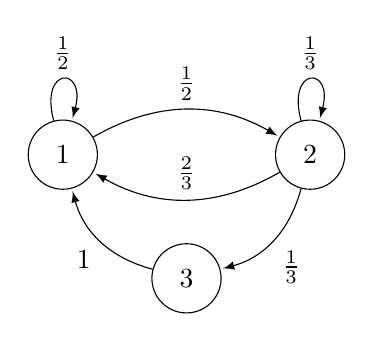
\begin{tikzpicture}

\node[state] (1) {1};
\node [right=of 1] (4) {};
\node[state, right=of 4] (2) {2};
\node[state, below=of 4] (3) {3};

\draw[every loop, >=latex]
(1) edge[loop above] node {$\frac{1}{2}$} (1)
(1) edge[bend left, auto=left] node {$\frac{1}{2}$} (2)
(2) edge[bend left, auto=left] node[above] {$\frac{2}{3}$} (1)
(2) edge[loop above] node {$\frac{1}{3}$} (2)
(2) edge[bend left, auto=left] node {$\frac{1}{3}$} (3)
(3) edge[bend left, auto=left] node {$1$} (1);

\end{tikzpicture}
\end{center}

In general, to calculate the probabilities associated with a Markov chain, we need to know two quantities.

\begin{itemize}
	\item \emph{The initial distribution}. We first need to know about the starting state of a Markov chain. This is described by the initial distribution $\lambda = (\lambda_i \mid i \in S)$, where $\lambda_i = \PP(X_0 = i)$.
	\item \emph{The transition probabilities}. We also need to know the probability of moving from a state $i \in S$ to a state $j \in S$. This is typically given by a \emph{transition matrix} $P = (P_{i, j} \mid i, j \in S)$ with $p_{i,j} = \PP(X_1 = j \mid X_0 = i)$.
\end{itemize}
These quantities are of course subject to some constraints, in that we require $\sum_{i \in S} \lambda_i = 1$ and the transition matrix $P$ must be \vocab{stochastic}, in that $\sum_{j \in S} P_{i, j} = 1$ for all $i \in S$.

If a Markov chain $X_n$ has initial distribution $\lambda$ and transition matrix $P$, we say that it is \vocab{$\markov(\lambda, P)$}.

Once we have these quantities, we can begin to actually establish various properties about the Markov chain, for example the probability that it goes through a given sequence of states.

\begin{theorem}[Probability of a Sequence of States]
	The sequence of random variables $X_n$ is $\markov(\lambda, P)$ if and only if
	$$
	\PP(X_0 = i_0, X_1 = i_1, \dots, X_n = i_n) = \lambda_{i_0}P_{i_0, i_1} \cdots P_{i_{n - 1}, i_n},
	$$
	for all $n \geq 0$ and $i_0, \dots, i_n \in S$.
\end{theorem}
\begin{proof}
	Let $A_k$ denote the event $\{X_k = i_k\}$. First suppose that $X_n$ is $\markov(\lambda, P)$. We prove the result holds by induction. For $n = 0$ this is true by definition. Then if it holds up to $n$, we have
	\begin{align*}
	\PP(A_0 \cap \cdots \cap A_n)  &= \PP(A_0 \cap \cdots \cap A_{n - 1})\PP(A_n \mid A_0 \cap \cdots \cap A_{n - 1}) \\
	&= \PP(A_0 \cap \cdots \cap A_{n - 1})\PP(A_n \mid A_{n - 1}) \\ 
	&= \left(\lambda_{i_0}P_{i_0, i_1} \cdots P_{i_{n - 2}, i_{n - 1}}\right)P_{i_{n - 1}, i_n},
\end{align*}
which completes our induction.

Conversely, suppose that the result holds. Then with $n = 0$ we get that the initial distribution of $X_n$ is $\lambda$. Then
$$
\PP(A_{n + 1} \mid A_{0} \cap \cdots \cap A_n) = \frac{\PP(A_0 \cap \cdots \cap A_{n + 1})}{\PP(A_0 \cap \cdots \cap A_{n})} = P_{i_{n}, i_{n + 1}}.
$$
Since this does not depend on $i_0, \dots, i_{n - 1}$, $X_n$ is a homogeneous Markov chain with transition matrix $P$, as required.
\end{proof}

Before moving on, let's get a feel for what is and isn't a Markov chain.

\begin{example}[Some Markov Chains, and a Non-Example]
	\begin{enumerate}[label=(\roman*)]
		\item \emph{An i.i.d.\ sequence}. If $X_0, X_1, X_2, \dots$ are independent and identically distributed random variables taking values in $S$, then $X_n$ is (rather boringly) a Markov chain: conditioning on the past changes nothing at all, and $P_{i, j} = \PP(X_1 = j)$ doesn't even depend on $i$.
		\item \emph{A random walk}. Let $\xi_1, \xi_2, \dots$ be i.i.d.\ integer-valued random variables and set $X_n = X_0 + \xi_1 + \cdots + \xi_n$. Then $X_n$ is a Markov chain on $\Z$, since given $X_n = x$, we have $X_{n + 1} = x + \xi_{n + 1}$, and $\xi_{n + 1}$ is independent of everything that came before. Random walks will be recurring characters throughout this course. A typical trajectory of the walk with steps $\xi_i = \pm 1$ looks like the following.

		\begin{center}
		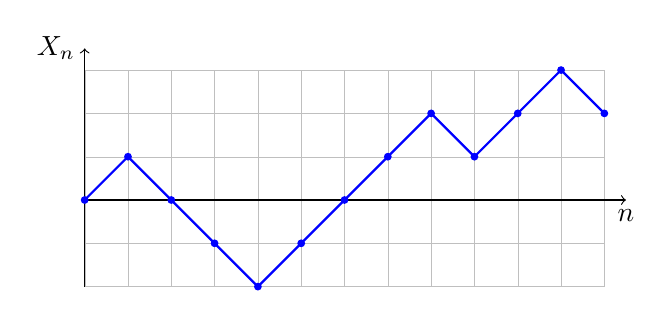
\begin{tikzpicture}[scale=0.55]
			\draw[ultra thin, color=lightgray] (0, -2) grid (12, 3);
			\draw[->] (0, 0) -- (12.5, 0) node[below] {$n$};
			\draw[->] (0, -2) -- (0, 3.5) node[left] {$X_n$};
			\draw[thick, color=blue]
				(0, 0) -- (1, 1) -- (2, 0) -- (3, -1) -- (4, -2) -- (5, -1) -- (6, 0)
				-- (7, 1) -- (8, 2) -- (9, 1) -- (10, 2) -- (11, 3) -- (12, 2);
			\foreach \x/\y in {0/0, 1/1, 2/0, 3/-1, 4/-2, 5/-1, 6/0, 7/1, 8/2, 9/1, 10/2, 11/3, 12/2}
				\fill[blue] (\x, \y) circle (0.09);
		\end{tikzpicture}
		\end{center}
		\item \emph{A non-example}. Let $X_n$ be the random walk above with steps $\pm 1$, and let $M_n = \max_{0 \leq k \leq n} X_k$ be its running maximum. Then $M_n$ is \emph{not} a Markov chain in general: knowing that $M_n = M_{n - 1} = m$ tells us the walk is currently strictly below its maximum, while knowing only $M_n = m$ leaves open the possibility $X_n = m$, and these lead to different probabilities that $M_{n + 1} = m + 1$. The past leaks information about the present position of the underlying walk, which the value of $M_n$ alone doesn't capture.
	\end{enumerate}
\end{example}

\begin{example}[Probability of a Path]
	Let's also see the previous theorem in action on the three-state chain drawn at the start of this section, with $S = \{1, 2, 3\}$ and initial distribution $\lambda = \delta_1$ (i.e.\ we start at state 1 with certainty). The probability that the chain follows the path $1 \to 2 \to 3 \to 1$ is
	$$
	\PP(X_0 = 1, X_1 = 2, X_2 = 3, X_3 = 1) = \lambda_1 P_{1, 2}P_{2, 3}P_{3, 1} = 1 \cdot \frac{1}{2} \cdot \frac{1}{3} \cdot 1 = \frac{1}{6}.
	$$
	Notice how the answer is just the product of the probabilities written on the arrows of the diagram, along the path taken -- this is a perfectly good way to think about the theorem.
\end{example}

\subsection{Simple Markov Property}

An important aspect of Markov chains is that they are \emph{memoryless}, in the future is independent of the past, conditional on the present. This is encapsulated in the \vocab{simple Markov property}.

\begin{theorem}[Simple Markov Property]
	Let $X_n$ be a Markov chain. Then conditional on $X_m = i$, the sequence of random variables $(X_{m + n})_{n \geq 0}$ is\footnote{Here $\delta_{ij}$ is 1 if $i = j$ and 0 otherwise.} $\markov(\delta_i, P)$, and is independent of $X_0, \dots, X_{m - 1}$.
\end{theorem}
\begin{proof}
	Given any event $H$ determined by $X_0, \dots, X_{m - 1}$, we want to show that for an event $F = \{X_m = i_m, \dots X_{m + n} = i_{m +n}\}$ we have
	$$
	\PP(H \cap F \mid X_m = i) = \delta_{ii_m}P_{i_m, i_{m + 1}} \cdots P_{i_{m + n-1}, i_{m + n}} \PP(H \mid X_m = i).
	$$
	Indeed, considering the case of $H = \{X_0 = i_0, \dots, X_m = i_m\}$ we have
	\begin{align*}
		\PP(H \cap F \mid X_m = i) &= \frac{\lambda_{i_0}P_{i_0, i_1} \cdots P_{i_{m - 1}, i}P_{i, i_{m + 1}} \cdots P_{i_{m + n - 1}, i_{m + n}}}{\PP(X_m = i)} \\
		&= \delta_{i i_m}P_{i, i_{m + 1}} \cdots P_{i_{m + n - 1}, i_{m + n}} \PP(H \mid X_m = i),
	\end{align*}
	as required. 
	
	Then for a general $H$, we can write it as the disjoint union $H = \bigcup_{k = 1}^{\infty} H_k$, and then the overall result follows by summing the above result for relevant $H_k$.
\end{proof}

\begin{remark}
	It is worth internalising what the simple Markov property really says: the chain, observed from time $m$ onwards, is a fresh copy of the Markov chain started from wherever it happened to be at time $m$ -- and this fresh copy doesn't care at all about the route taken to get there. For instance, for any states $i, j, k$,
	$$
	\PP(X_5 = j \mid X_3 = i, X_0 = k) = \PP(X_5 = j \mid X_3 = i) = \PP(X_2 = j \mid X_0 = i),
	$$
	so conditional probabilities of the future can always be `re-rooted' to time zero. We will use manipulations of this sort constantly, and usually without comment.
\end{remark}

\subsection{Transition Probabilities}

We are now going to address how to find the probability that a Markov chain is in a given state after $n$ steps.
The core idea of this section is that we will be able to reduce such questions into questions about the transition matrix that we introduced earlier.

Recall that if $X_n$ is a Markov chain with transition matrix $P$, then $P_{i, j}$ was the probability of moving from the state $i$ to the state $j$. We call these the \vocab{one-step transition probabilities}. We can generalize this slightly.

\begin{definition}[$n$-Step Transition Probabilities]
	For a Markov chain $X_n$, the \vocab{$n$-step transition probabilities} are given by
	$$
	p_{i, j}(n) = \PP(X_n = j \mid X_0 = i).
	$$
\end{definition}

These $n$-step transition probabilities naturally form the \vocab{$n$-step transition matrix} $P(n) = (p_{i, j}(n) \mid i, j \in S)$. The nice thing about writing these transition probabilities as a matrix is that they satisfy a lovely set of equations that relate extremely well to matrix algebra.

\begin{theorem}[Chapman-Kolmogorov Equations]
	We have that
	$$
	p_{i, j}(n + m) = \sum_{k \in S} p_{i, k}(n)p_{k, j}(m),
	$$
	where $i, j \in S$ and $m, n \geq 0$. In particular, $P(m + n) = P(m)P(n)$.
\end{theorem}
\begin{proof}
	Using the partition theorem and simple Markov property,
	\begin{align*}
		p_{i, j}(n + m) &= \PP(X_{n + m} = j \mid X_0 = i) \\
		&= \sum_{k \in S} \PP(X_{m + n} = j \mid X_n = k, X_0 = i) \PP(X_n = k \mid X_0 = i) \\
		&= \sum_{k \in S} \PP(X_{m + n} = j \mid X_n = k) \PP(X_n = k \mid X_0 = i) \\
		&= \sum_{k \in S} p_{i, k}(n) p_{k, j}(m).
	\end{align*}
\end{proof}

So, if we have some $n$-step transition matrix $P(n)$, the above result shows us that it satisfies $P(n) = P^n$. This reduces our problem to just this:

\begin{center}
	\color{blue}
	To compute $p_{i, j}(n)$, we can compute powers of\\ the transition matrix, and take $(P^n)_{i, j}$.
\end{center}

In general, this makes our problem significantly easier, and if the state space is finite, we can use tools from linear algebra such as diagonalisation.

\begin{example}[Predicting the Weather]
	Suppose the weather in Cambridge is sunny, cloudy or rainy, and that tomorrow's weather depends only on today's\footnote{A bold modelling assumption, but this is a mathematics course.}, according to the transition matrix
	$$
	P = \begin{pmatrix}
		1/2 & 1/3 & 1/6 \\
		1/4 & 1/2 & 1/4 \\
		1/4 & 1/4 & 1/2
	\end{pmatrix},
	$$
	where the states are (sunny, cloudy, rainy) in that order. If it is sunny today, what is the probability that it rains two days from now?

	By our discussion above, this is just the matrix entry
	$$
	(P^2)_{1, 3} = \sum_{k = 1}^{3} P_{1, k}P_{k, 3} = \frac{1}{2}\cdot\frac{1}{6} + \frac{1}{3}\cdot\frac{1}{4} + \frac{1}{6}\cdot\frac{1}{2} = \frac{1}{12} + \frac{1}{12} + \frac{1}{12} = \frac{1}{4},
	$$
	where the three terms account for the three possible weathers tomorrow. There is nothing special about two days -- the probability for any horizon $n$ is read off from $P^n$, computable by repeated squaring or by diagonalisation as described above.
\end{example}

While we are speaking the language of matrices, it is worth recording what happens when the starting state is itself random. Treating the initial distribution $\lambda$ as a \emph{row vector}, the distribution of the chain at time $n$ is obtained by simply multiplying by powers of $P$.

\begin{proposition}[Distribution at Time $n$]
	Let $X_n$ be $\markov(\lambda, P)$. Then for all $n \geq 0$ and $j \in S$,
	$$
	\PP(X_n = j) = (\lambda P^n)_j.
	$$
\end{proposition}
\begin{proof}
	Conditioning on the starting state and using the previous result,
	$$
	\PP(X_n = j) = \sum_{i \in S} \PP(X_0 = i)\PP(X_n = j \mid X_0 = i) = \sum_{i \in S} \lambda_i (P^n)_{i, j} = (\lambda P^n)_j. \qedhere
	$$
\end{proof}

So the entire distributional evolution of a Markov chain is captured by the linear algebra of the pair $(\lambda, P)$ -- a fact we will lean on constantly, and which will become especially interesting when we ask what happens as $n \rightarrow \infty$ later in the course.

\begin{example}[Computing Transition Probabilities]
	Let $\alpha, \beta \in (0, 1)$. 
	Consider the Markov chain $X_n$ with states $S = \{1, 2\}$, with transition matrix 
	$$
	P = \begin{pmatrix}
		1 - \alpha & \alpha \\
		\beta & 1 - \beta
	\end{pmatrix}.
	$$
	A diagram of this Markov chain is shown below.
	\begin{center}
	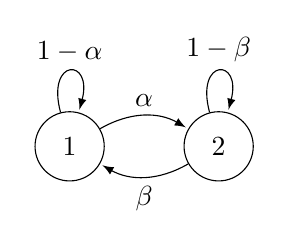
\begin{tikzpicture}

	\node[state] (1) {1};
	\node[state, right=of 1] (2) {2};

	\draw[every loop, >=latex]
	(1) edge[loop above] node {$1 - \alpha$} (1)
	(1) edge[bend left, auto=left] node {$\alpha$} (2)
	(2) edge[bend left, auto=left] node {$\beta$} (1)
	(2) edge[loop above] node {$1 -\beta$} (2);

	\end{tikzpicture}
	\end{center}

	We want to find the $n$-step transition probabilities.

	\textbf{Method 1} (Difference Equations). We are first going to find $p_{1, 1}(n)$ using a `bare-hands' method. By the Chapman-Kolmogorov equations (that is, conditioning on $X_n$) we have
	\begin{align*}
		p_{1, 1}(n + 1) &= p_{1, 1}(n)p_{1, 1}(1) + p_{1, 2}(n) p_{2, 1}(1) \\
		&= (1 - \alpha)p_{1, 1}(n) + \beta p_{1, 2}(n) \\
		&= (1 - \alpha)p_{1, 1}(n) + \beta (1 - p_{1, 1}(n)) \\
		&= p_{1, 1}(n)(1 - \alpha - \beta) + \beta.
	\end{align*}
	This is a recurrence relation which we can then solve using the boundary condition $p_{1, 1}(0) = 1$ to get
	$$
		p_{1, 1}(n) = \begin{cases}
			\frac{\beta}{\alpha+\beta}+\frac{\alpha}{\alpha+\beta} \cdot(1-\alpha-\beta)^{n} &\mbox{if } \alpha + \beta > 0, \\
			1 &\mbox{if } \alpha + \beta = 0.
		   \end{cases}
	$$

	\textbf{Method 2} (Diagonalisation). An alternative solution uses some tools from matrix algebra. To calculate the $n$-step transition matrix $P^n$, we are going to diagonalise $P$.

	The eigenvalues of $P$ are given by the solutions to $\det(P - \mu I) = 0$, which are $\{1, 1 - \alpha - \beta\}$. Thus for some invertible matrix $U$ we have
	$$
	P = U^{-1}\begin{pmatrix}
		1 & 0 \\ 0 & 1 - \alpha - \beta
	\end{pmatrix}U \quad \text{and} \quad P^n = U^{-1} \begin{pmatrix}
		1 & 0 \\ 0 & (1 - \alpha - \beta)^n
	\end{pmatrix}U.
	$$
	Thus $p_{1, 1}(n) = A + B(1 - \alpha - \beta)^n$, for constants $A$ and $B$. We can find these by noting the boundary conditions $p_{1, 1}(0) = 1$ and $p_{1, 1}(1) = 1 - \alpha$, giving
	$$
		p_{1, 1}(n) = \begin{cases}
			\frac{\beta}{\alpha+\beta}+\frac{\alpha}{\alpha+\beta} \cdot(1-\alpha-\beta)^{n} &\mbox{if } \alpha + \beta > 0, \\
			1 &\mbox{if } \alpha + \beta = 0.
		   \end{cases}
	$$
\end{example}

In general, if the state space of a Markov chain is finite with $|S| = k$, then $P$ is a $k \times k$ matrix with eigenvalues $\mu_1, \dots, \mu_k$.

If \emph{all of the eigenvalues are distinct}, then $P$ is diagonalisable, and we can write
$$
P = U^{-1} \begin{pmatrix}
	\mu_1 & \cdots & 0 \\
	0 & \ddots & 0 \\
	0 & \cdots & \mu_k
\end{pmatrix} U \quad \text{and} \quad P^n = U^{-1} \begin{pmatrix}
	\mu_1^n & \cdots & 0 \\
	0 & \ddots & 0 \\
	0 & \cdots & \mu_k^n
\end{pmatrix} U,
$$
and $p_{i,j} = a_1 \mu_1^n + \cdots + a_k \mu_k^n$, for some constants $a_1, \dots, a_k$, which are determined by the boundary conditions.

If some eigenvalue $\mu_k$ is complex, then it's conjugate is also an eigenvalue, so if $\mu_k = re^{i \theta}$ we have also the eigenvalue $\overline{\mu_k} = re^{-i \theta}$, and we can write
$$
p_{i, j} = a_1 \mu_1^n + \cdots + a_{k - 2}\mu_{k - 2}^n + a_{k - 1}r^n \cos(n \theta) + a_k r^n \sin (n \theta),
$$
since $p_{i, j}$ is real and so all of the imaginary parts must cancel out.


If \emph{some eigenvalues repeat}, then the situation is slightly more complicated. If an eigenvalue $\mu_k$ has multiplicity $m$, we can simply replace $a_k$ by a degree $m$ polynomial in $n$\footnote{This comes from considering the Jordan Normal form of the transition matrix.}. 


\begin{example}[Transition Matrix with Complex Eigenvalues]
	Consider the Markov chain $X_n$ with states $S = \{1, 2, 3\}$ as shown in the diagram below. We want to find the $n$-step transition probability $p_{i, i}(n)$.
	\begin{center}
	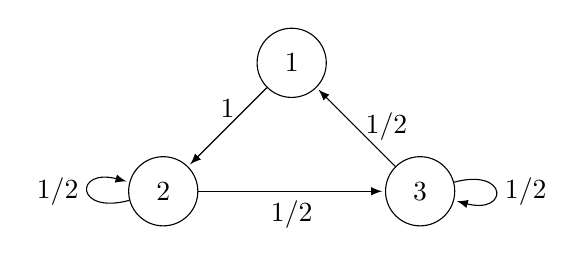
\begin{tikzpicture}

	\node[state] (1) {1};
	\node[state, below left=of 1] (2) {2};
	\node[state, below right=of 1] (3) {3};

	\draw[every loop, >=latex]
	(1) edge[above] node {$1$} (2)
	(2) edge[loop left] node {$1/2$} (2)
	(2) edge[below] node {$1/2$} (3)
	(3) edge[loop right] node {$1/2$} (3)
	(3) edge[right] node {$1/2$} (1);

	\end{tikzpicture}
	\end{center}

	This Markov chain has the transition matrix
	$$
	P = \begin{pmatrix}
		0 & 1 & 0 \\
		0 & 1/2 & 1/2 \\ 
		1/2 & 0 & 1/2
	\end{pmatrix},
	$$
	which has distinct eigenvalues $\{1, i/2, -i/2\}$.

	We can rewrite the complex eigenvalues using trigonometric functions as
	\begin{align*}
		\frac{i}{2} &= \cos \frac{\pi}{2} + i \sin \frac{\pi}{2}, \\ 
		-\frac{i}{2} &= \cos \frac{\pi}{2} - i \sin \frac{\pi}{2}.
	\end{align*}

	The general form for $p_{1,1}(n)$ is then given by
	$$
	p_{1,1}(n) = A + B \cdot \left(\frac{1}{2}\right)^n \cos \left(\frac{n \pi}{2}\right) + C \cdot \left(\frac{1}{2}\right)^n \sin\left(\frac{n \pi}{2}\right).
	$$
	The boundary conditions can be computed by hand as
	$p_{1,1}(0) = 1$, $p_{1,1}(1) = 0$ and $p_{1,1}(2) = 0$. This allows us to solve for $A$, $B$ and $C$ to get
	$$
	p_{1,1}(n) = \frac{1}{5} + \left(\frac{1}{2}\right)^n \left(\frac{4}{5}\cos\left(\frac{n \pi}{2}\right) - \frac{2}{5} \sin \left(\frac{n \pi}{2}\right)\right).
	$$
\end{example}

\section{Class Structure}


\subsection{Communicating Classes}

In Graph Theory, one can often make a problem easier by looking at the \emph{connected components} of the graph, effectively splitting it up into smaller disconnected chunks which are easier to understand on their own. 
This has a natural analogue in the study of Markov chains,\footnote{Indeed, one can view a Markov chain as a labelled directed graph, and then apply the same connected components argument to obtain the theory shown here.} where we consider which states can interact.

\begin{definition}[Communication]
	Let $X_n$ be a Markov chain. For $i, j \in S$, we say that $i$ \vocab{leads to} $j$, written $i \rightarrow j$, if $p_{i, j}(n) > 0$ for some $n \geq 0$.

	If $i \rightarrow j$ and $j \rightarrow i$, we say that $i$ and $j$ \vocab{communicate}, and write $i \leftrightarrow j$.
\end{definition}

We can use this idea of communication to break up our state space by noting that communication is an equivalence relation.

\begin{theorem}[Communication is an Equivalence Relation]
The relation $\leftrightarrow$ is an equivalence relation on $S$.
\end{theorem}
\begin{proof}
	For any $i \in S$, $p_{i, i}(0) = 1$ and thus $i \leftrightarrow i$, so the relation is reflexive. The relation is symmetric by definition, so we are just left to check transitivity.

	Let $i, j, k \in S$, and suppose that $i \leftrightarrow j$ and $j \leftrightarrow k$. Then there exists $m, n \geq 0$ such that $p_{i, j}(n) > 0$ and $p_{j, k}(m) > 0$. Then by the Chapman-Kolmogorov equations,
	\begin{align*}
		p_{i, k}(m + n) = \sum_{l \in S}p_{i, l}(m)p_{l, k}(n) \geq p_{i, j}(n) p_{j, k}(m) > 0,
	\end{align*}
	so $i \rightarrow k$. By the same argument $k \rightarrow i$, and thus $\leftrightarrow$ is transitive.
\end{proof}

Because communication is an equivalence relation, it partitions the state space.

\begin{definition}[Communicating Classes]
	The equivalence classes induced by $\longleftrightarrow$ on $S$ are called \vocab{communicating classes}.
\end{definition}

Because communication is really a notion about directed graphs (and not \emph{really} about individual probabilities), it's usually relatively easy to identify the communicating classes from the diagram of a Markov chain.

For example, the Markov chain below has its communicating classes coloured (and the transition probabilities are not labelled, as they are not needed to infer the communicating classes, aside from knowing they are non-zero along each edge).

\begin{center}
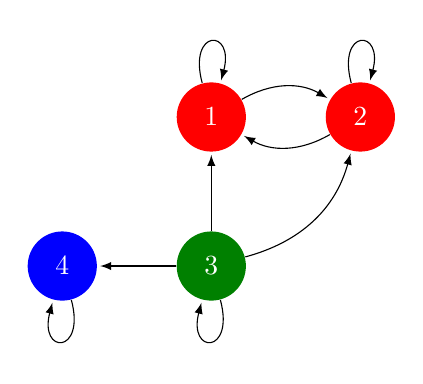
\begin{tikzpicture}

\tikzstyle{every state}=[fill,draw=none,blue,text=white]
\tikzstyle{accepting}=[green!50!black,text=white]
\tikzstyle{initial}= [red,text=white]

\node[state, initial] (1) {1};
\node[state, initial, right=of 1] (2) {2};
\node[state, accepting, below=of 1] (3) {3};
\node[state, left=of 3] (4) {4};

\draw[every loop, >=latex]
(1) edge[loop above] (1)
(1) edge[bend left, above] (2)
(2) edge[loop above] (2)
(2) edge[bend left, below] (1)
(3) edge[left] (1)
(3) edge[below] (4)
(3) edge[bend right, right] (2)
(3) edge[loop below] (3)
(4) edge[loop below] (4);

\end{tikzpicture}
\end{center}

In the Markov chain above, we can see that there are a few different ways that communicating classes can appear.

A communicating class $C$ is \vocab{closed} if there is no way to leave it, in that if $i \in C$ and $i \rightarrow j$, then $j$ in $C$. For example, in the Markov chain above, the communicating class $\{1, 2\}$ is closed.

A state $i \in S$ is \vocab{absorbing} if there is no way to leave that state, that is, $\{i\}$ is a communicating class. In the Markov chain above, $4$ is absorbing.

If a Markov chain has only one communicating class, we call it \vocab{irreducible}, as we cannot split it into smaller parts in this way.

Let's put these definitions to use on a concrete example.

\begin{example}[Finding the Communicating Classes]
	Consider the Markov chain on $S = \{1, 2, 3, 4, 5\}$ with transition matrix
	$$
	P = \begin{pmatrix}
		1/2 & 1/2 & 0 & 0 & 0 \\
		1 & 0 & 0 & 0 & 0 \\
		1/3 & 0 & 1/3 & 1/3 & 0 \\
		0 & 0 & 0 & 1/2 & 1/2 \\
		0 & 0 & 0 & 1 & 0
	\end{pmatrix}.
	$$
	Drawing the diagram (which, as we said, is usually the right move) gives the following.

	\begin{center}
	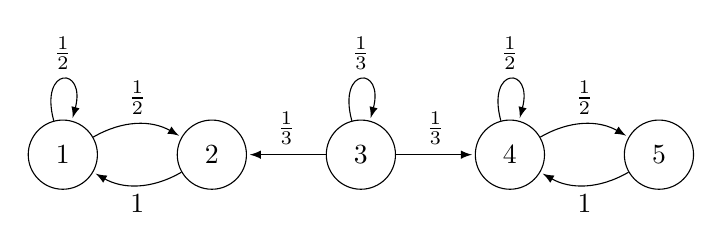
\begin{tikzpicture}

	\node[state] (1) {1};
	\node[state, right=of 1] (2) {2};
	\node[state, right=of 2] (3) {3};
	\node[state, right=of 3] (4) {4};
	\node[state, right=of 4] (5) {5};

	\draw[every loop, >=latex]
	(1) edge[loop above] node {$\frac{1}{2}$} (1)
	(1) edge[bend left, auto=left] node {$\frac{1}{2}$} (2)
	(2) edge[bend left, auto=left] node {$1$} (1)
	(3) edge[auto=right] node[above] {$\frac{1}{3}$} (2)
	(3) edge[loop above] node {$\frac{1}{3}$} (3)
	(3) edge[auto=left] node {$\frac{1}{3}$} (4)
	(4) edge[loop above] node {$\frac{1}{2}$} (4)
	(4) edge[bend left, auto=left] node {$\frac{1}{2}$} (5)
	(5) edge[bend left, auto=left] node {$1$} (4);

	\end{tikzpicture}
	\end{center}

	We can now just read off the class structure. States 1 and 2 communicate (each leads to the other in one step), and nothing outside $\{1, 2\}$ can be reached from them, so $\{1, 2\}$ is a \emph{closed} communicating class. Similarly $\{4, 5\}$ is a closed class. State 3 leads to state 2 and state 4, but neither leads back to 3, so $\{3\}$ is a communicating class by itself, and it is \emph{not} closed.

	This chain is not irreducible -- it has three communicating classes. Intuitively, the chain will linger at 3 for a (geometrically distributed) while, and then fall either left into $\{1, 2\}$ or right into $\{4, 5\}$, where it will remain trapped forever. Computing the probability of each of these outcomes is a matter of \emph{hitting probabilities}, which is exactly the business of the next section.
\end{example}

\section{Hitting Times, Stopping Times and Absorption Probabilities}

\subsection{Hitting Times}

When studying Markov chains, a frequently occurring question is `\emph{how long does it take to reach a given state $i \in S$?}', a concept which we formulate as the \emph{hitting time}.

\begin{definition}[Hitting Time]
	Let $X_n$ be a Markov chain.
	The \vocab{hitting time} of some subset of states $A \subseteq S$ is the random variable $T_A$, which is the least $n$ for which $X_n \in A$.
	In particular,
	$$
	T_A = \inf\{n \geq 0 \mid X_n \in A\},
	$$
	where this may be $\infty$ if $X_n \not \in A$ for all $n \geq 0$.
\end{definition}

In this section, we will also look some related quantities, such as the \emph{hitting probability} and \emph{mean hitting time}.

\begin{definition}[Hitting Probability]
	Let $X_n$ be a Markov chain, and let $A \subseteq S$ be some subset of states.
	The \vocab{hitting probability} $h^A_i$ of $A$ is the probability that $X_n$ eventually reaches a state in $A$, given $X_0 = i$. That is,
	$$
	h^A_i = \PP(T_A < \infty \mid X_0 = i),
	$$
	where $i \in S$.
\end{definition}

\begin{definition}[Mean Hitting Time]
	Let $X_n$ be a Markov chain, and let $A \subseteq S$ be some subset of states.
	The \vocab{mean hitting time} $k^A_i$ of $A$ is the expected number of steps taken for $X_n$ to reach a state in $A$, given $X_0 = i$. That is,
	$$
	k^A_i = \EE[T_A \mid X_0 = i],
	$$
	where $i \in S$. We note that this may be $\infty$.
\end{definition}

So how do we go about calculating these quantities? An intuitive way is to try and consider what happens as we move from one state to another, as we will see in the example below.

\begin{example}[Computing Hitting Probabilities and Mean Hitting Times]
	Consider the Markov chain in the diagram below.
	\begin{center}
		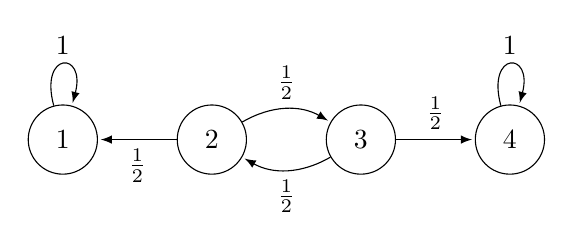
\begin{tikzpicture}
		
		\node[state] (1) {1};
		\node[state, right=of 1] (2) {2};
		\node[state, right=of 2] (3) {3};
		\node[state, right=of 3] (4) {4};
		
		\draw[every loop, >=latex]
		(1) edge[loop above] node {$1$} (1)
		(2) edge[auto=left] node {$\frac{1}{2}$} (1)
		(2) edge[bend left, auto=left] node {$\frac{1}{2}$} (3)
		(3) edge[bend left, auto=left] node {$\frac{1}{2}$} (2)
		(3) edge[auto=left] node {$\frac{1}{2}$} (4)
		(4) edge[loop above] node {$1$} (4);
		
		\end{tikzpicture}
		\end{center}

		Suppose we took $A = \{4\}$ and wanted to find the hitting probability $h_2^A = \PP(T_A < \infty \mid X_0 = 2)$. One might intuitively suppose that
		\begin{align*}
			h_2^A &= P_{2, 3} h_3^A = \frac{1}{2} h_3^A, \\
			h_3^A &= P_{3, 2} \cdot h_2^A + P_{3, 4} \cdot h_4^A = \frac{1}{2} \cdot h_2^A + \frac{1}{2}.
		\end{align*}
		which when solved gives us $h_2^A = 1/3$.

		Alternatively, if we took $B = \{1, 4\}$ and wanted to find the mean hitting time $k_2^B$, we could again try the intuitive approach of writing
		$$
		k_2^B = 1 + \frac{1}{2}k_3^B,
		$$
		and noting that $k_3^B = k_2^B$ by symmetry, giving $k_2^B = 2$.
\end{example}

In the computations above, we really should check that these are valid methods (though it \emph{really is} quite intuitive).

\begin{theorem}[Computing Hitting Probabilities]
	Let $A \subseteq S$. Then the set of hitting probabilities $h^A = (h_i^A \mid i \in S)$ is the minimal\footnote{Minimal in that if $x$ is another non-negative solution, then $x_i \geq h_i^A$ for all $i \in S$.} non-negative solution to the equations
	\begin{align*}
		h_i^A = \begin{cases}
			1 &\mbox{if } i  \in A, \\
			\sum_{j \in S} P_{i, j} h_j^A &\mbox{if } i \not \in A.
		   \end{cases}
	\end{align*}
\end{theorem}
\begin{proof}
	We first check that $h_i$ solves this system. Clearly if $i \in A$, then $h_i^A = 1$, so take $i \in S\backslash A$. Then conditioning on the first step in the chain,
	\begin{align*}
		h_i^A &= \sum_{j \in S} P_{i, j} \PP(T_A < \infty \mid X_0 = i, X_1 = j)  \\
		&= \sum_{j \in S} P_{i, j} h_j^A,
	\end{align*}
	by the simple Markov property. So $h_i$ does indeed solve this system.

	We now check minimality. Let $x = (x_i \mid i \in S)$ be another non-negative solution. For $i \in A$, we have $x_i = h^A_i = 1$, so that holds. Then for $i \in S \backslash A$, since $x$ satisfies the system of equations we can write
	\begin{equation}\label{mc-eq:1}
		x_i = \sum_{j \in S}P_{i, j} x_j = \sum_{j \in A} P_{i, j} x_j + \sum_{j \in S \backslash A} P_{i, j} x_j. \tag{$\dagger$}
	\end{equation}
	Then with $x_j = 1$ for $j \in A$ and $x \geq 0$, we have
	\begin{align*}
		x_i \geq \sum_{j \in A} P_{i, j} = \PP(X_1 \in A \mid X_0 = i) = \PP(T_A < 2 \mid X_0 = i).
	\end{align*}
	Similarily, expanding \eqref{mc-eq:1}, we have
	\begin{align*}
	x_i &= \PP(X_1 \in A \mid X_0 = i) + \sum_{j \in S \backslash A} P_{i, j} \left(\sum_{k \in A} P_{j, k} x_k + \sum_{k \in S \backslash A} P_{j, k} x_k\right) \\
		&\geq \PP(X_1 \in A \mid X_0 = i) + \PP(X_1 \not \in A, X_2 \in A \mid X_0 = i) \\
		&= \PP(T_A < 3 \mid X_0 = i).
	\end{align*}
	We can repeat this argument to eventually establish that $x_i \geq \PP(T_A < n \mid X_0 = i)$, for all $n \geq 0$. Then as $n \rightarrow \infty$, we have $x_i \geq \PP(T_A < \infty \mid X_0 = i)$, as required.
\end{proof}

Let's also settle a question we left dangling at the end of the previous section: for the five-state chain whose classes were $\{1, 2\}$ (closed), $\{3\}$ and $\{4, 5\}$ (closed), where does the chain end up when started from state 3?

\begin{example}[Absorption Probabilities]
	Take $A = \{1, 2\}$, and let $h_i = h_i^A$. We have $h_1 = h_2 = 1$, and since states 4 and 5 can never reach $A$, also $h_4 = h_5 = 0$. From state 3, the chain moves to each of states 2, 3, 4 with probability $1/3$, so
	$$
	h_3 = \frac{1}{3}h_2 + \frac{1}{3}h_3 + \frac{1}{3}h_4 = \frac{1}{3} + \frac{1}{3}h_3,
	$$
	giving $h_3 = 1/2$. So the chain started from 3 is absorbed into $\{1, 2\}$ or into $\{4, 5\}$ with probability $1/2$ each -- which makes sense, as the two escape routes from state 3 are equally likely, and dawdling at 3 doesn't favour either.
\end{example}

This method of computing hitting probabilities is perfectly valid on Markov chains with infinite state spaces.

\begin{example}[Hitting Probabilities on an Infinite State Space]
	Consider the Markov chain with states $S = \{0, 1, \dots\}$ such that $P_{0, 1} = 1$, and
	$$
	P_{i, i+1} = p, \quad P_{i, i - 1} = q \quad \text{for all } i \geq 1,
	$$ 
	where $p, q \in (0, 1)$ with $p + q = 1$.

	\begin{center}
		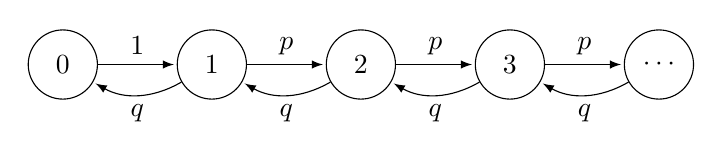
\begin{tikzpicture}

		\node[state] (1) {0};
		\node[state, right=of 1] (2) {1};
		\node[state, right=of 2] (3) {2};
		\node[state, right=of 3] (4) {3};
		\node[state, right=of 4] (5) {$\cdots$};

		\draw[every loop, >=latex]
		(1) edge[above] node {1} (2)
		(2) edge[above] node {$p$} (3)
		(3) edge[above] node {$p$} (4)
		(4) edge[above] node {$p$} (5)
		(2) edge[bend left, below] node {$q$} (1)
		(3) edge[bend left, below] node {$q$} (2)
		(4) edge[bend left, below] node {$q$} (3)
		(5) edge[bend left, below] node {$q$} (4);
		\end{tikzpicture}
		\end{center}

	Let $h_i = \PP(T_0 < \infty \mid X_0 = i)$, and suppose that $p \neq q$. Then we clearly have $h_0 = 1$, and generally we can write down the recurrence 
	$$
		h_i = p h_{i + 1} + qh_{i - 1}.
	$$
	This then implies $p(h_{i + 1} - h_i) = q(h_{i} - h_{i - 1})$, so that
	$$
		h_{i+1} - h_{i}  = \left(\frac{q}{p}\right)^i (h_1 - 1).
	$$
	This inspires us to write $h_i$ as a telescoping sum
	\begin{align*}
		h_i &= \sum_{j = 1}^i (h_j - h_{j - 1}) + 1  \\
			&= (h_1 - 1) \sum_{j = 1}^i \left(\frac{q}{p}\right)^j + 1,
	\end{align*}
	which gives us our general solution $h_i = a + b(q/p)^i$, which we can then solve.

	In the case that $q > p$, then in order for $h_i$ to be the minimal solution, we need to have $a = 1$ and $b = 0$, so $h_i = 1$.
\end{example}

We also need to check that our method for calculating the mean hitting time was valid.

\begin{theorem}[Computing Mean Hitting Times]
	Let $A \subseteq S$. Then the set of mean hitting times $k^A = (k_i^A \mid i \in S)$ is the minimal non-negative solution to the equations
	\begin{align*}
		k_i^A = \begin{cases}
			0 &\mbox{if } i  \in A, \\
			1 + \sum_{j \in S\backslash A} P_{i, j} k_j^A &\mbox{if } i \not \in A.
		   \end{cases}
	\end{align*}
\end{theorem}
\begin{proof}
	We first check that $k_i$ solves this system. Clearly if $i \in A$, then $k_i^A = 0$, so take $i \in S \backslash A$. Then conditioning on the first step in the chain,
	\begin{align*}
		k_i^A &= \sum_{j \in S} P_{i, j}\EE[T_A \mid X_0 = i, X_1 = j]  \\
		&= \sum_{j \in S} P_{i, j}(1 + \EE[T_A \mid X_0 = j]) \\
		&= 1 + \sum_{j \in S} P_{i, j} k_j^A, 	
	\end{align*}
	which is equivalent to our original sum.

	We now show that the solution is minimal. Let $y = (y_i \mid i \in S)$ be another non-negative solution. Then for $i \in A$ we have $y_i = k_i^A = 0$, so consider $i \in S \backslash A$. We can then write
	\begin{align*}
	y_i &= 1 + \sum_{j \in S \backslash A} P_{i, j} y_j  \\
	&= 1 + \sum_{j \in S \backslash A} P_{i, j}\left(1 + \sum_{k \in S \backslash A} P_{j, k} y_k\right) \\
	&\geq \PP(T_A \geq 1 \mid X_0 = i) + \PP(T_A \geq 2 \mid X_0 = i).
	\end{align*}
	By iterating this, we obtain
	$$
	y_i \geq \sum_{m = 1}^n \PP(T_A \geq m \mid X_0 = i),
	$$
	and taking the limit as $n \rightarrow \infty$, this gives
	$$
	y_i \geq \sum_{m = 1}^{\infty} \PP(T_A \geq m \mid X_0 = i) = k_i^A,
	$$
	where we note that for a random variable $M$ taking non-negative integer values we have $\EE[M] = \sum_{m = 1}^{\infty} \PP(M \geq m).$
\end{proof}

So it does work, how lovely.

\subsection{Gambler's Ruin}

Let's now put these tools to work on one of the oldest problems in probability. A gambler walks into a casino with $\pounds i$ in their pocket, and repeatedly plays a game in which they win $\pounds 1$ with probability $p$ and lose $\pounds 1$ with probability $q = 1 - p$. The gambler has no self-control, and will keep playing until they go bankrupt. We'd like to know the probability that this happens\footnote{Spoiler: unless the game is rigged in the gambler's favour, it happens with probability 1. The house always wins.}.

We can model this situation with a Markov chain on the states $S = \{0, 1, 2, \dots\}$, where the state tracks the gambler's current fortune. We set
$$
P_{i, i + 1} = p, \quad P_{i, i - 1} = q \quad \text{for all } i \geq 1,
$$
and $P_{0, 0} = 1$, since a bankrupt gambler can no longer play. A diagram of this chain is shown below.

\begin{center}
	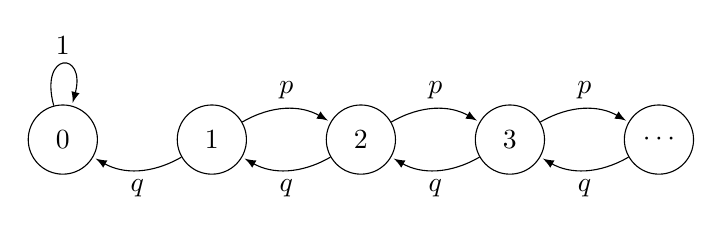
\begin{tikzpicture}

	\node[state] (0) {0};
	\node[state, right=of 0] (1) {1};
	\node[state, right=of 1] (2) {2};
	\node[state, right=of 2] (3) {3};
	\node[state, right=of 3] (4) {$\cdots$};

	\draw[every loop, >=latex]
	(0) edge[loop above] node {1} (0)
	(1) edge[bend left, above] node {$p$} (2)
	(2) edge[bend left, above] node {$p$} (3)
	(3) edge[bend left, above] node {$p$} (4)
	(1) edge[bend left, below] node {$q$} (0)
	(2) edge[bend left, below] node {$q$} (1)
	(3) edge[bend left, below] node {$q$} (2)
	(4) edge[bend left, below] node {$q$} (3);
	\end{tikzpicture}
	\end{center}

The probability of ruin starting from a fortune of $i$ is exactly the hitting probability $h_i = h_i^{\{0\}}$, so we can use the machinery of the previous section. We know that $h = (h_i \mid i \in S)$ is the minimal non-negative solution to
$$
h_0 = 1, \qquad h_i = p h_{i + 1} + q h_{i - 1} \text{ for } i \geq 1.
$$

This is a linear difference equation, which we know how to solve. Suppose first that $p \neq q$. Then the general solution is
$$
h_i = A + B \left(\frac{q}{p}\right)^i,
$$
and the boundary condition $h_0 = 1$ forces $A + B = 1$.

If $p < q$ (the game is stacked against the gambler, as it usually is), then $(q/p)^i \rightarrow \infty$ as $i \rightarrow \infty$, and since $h_i \in [0, 1]$ is a probability we must have $B = 0$. Thus $h_i = 1$ for all $i$ -- \emph{the gambler is certain to go bankrupt}.

If instead $p > q$, then substituting $B = 1 - A$ gives
$$
h_i = \left(\frac{q}{p}\right)^i + A\left(1 - \left(\frac{q}{p}\right)^i\right),
$$
which is a genuine non-negative solution for any $A \geq 0$. Minimality then tells us to take $A = 0$, giving
$$
h_i = \left(\frac{q}{p}\right)^i.
$$
So with a favourable game the gambler has a positive chance $1 - (q/p)^i$ of playing forever.

We are left with the fair case $p = q = 1/2$. Here the general solution to the difference equation is $h_i = A + Bi$, and for $h_i$ to remain in $[0, 1]$ for all $i$ we need $B = 0$, so $h_0 = 1$ forces $h_i = 1$ for all $i$. That is, \emph{even in a perfectly fair game, ruin is certain}.

The same circle of ideas handles the case where the gambler resolves to walk away upon reaching some target fortune.

\begin{example}[Gambling Against a Target]
	Suppose the game is fair ($p = q = 1/2$), and the gambler starts with $\pounds i$ but will stop when they reach either $\pounds 0$ or a target of $\pounds N$, where $0 \leq i \leq N$. Now both 0 and $N$ are absorbing, and the interesting quantities are the ruin probability $h_i = h_i^{\{0\}}$ and the expected duration of the game $k_i = k_i^{\{0, N\}}$.

	\begin{center}
	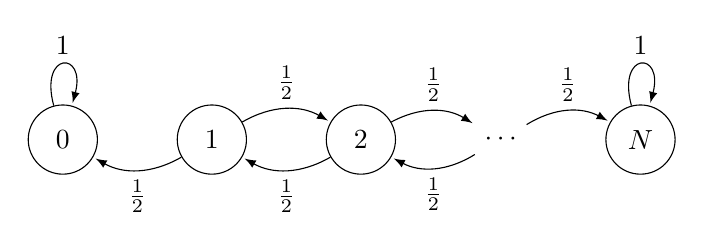
\begin{tikzpicture}

	\node[state] (0) {0};
	\node[state, right=of 0] (1) {1};
	\node[state, right=of 1] (2) {2};
	\node[right=of 2] (3) {$\cdots$};
	\node[state, right=of 3] (4) {$N$};

	\draw[every loop, >=latex]
	(0) edge[loop above] node {1} (0)
	(4) edge[loop above] node {1} (4)
	(1) edge[bend left, above] node {$\frac{1}{2}$} (2)
	(2) edge[bend left, above] node {$\frac{1}{2}$} (3)
	(3) edge[bend left, above] node {$\frac{1}{2}$} (4)
	(1) edge[bend left, below] node {$\frac{1}{2}$} (0)
	(2) edge[bend left, below] node {$\frac{1}{2}$} (1)
	(3) edge[bend left, below] node {$\frac{1}{2}$} (2);

	\end{tikzpicture}
	\end{center}

	For the ruin probability, we have the same difference equation $h_i = \frac{1}{2}h_{i - 1} + \frac{1}{2}h_{i + 1}$ for $0 < i < N$, but now with \emph{two} boundary conditions $h_0 = 1$ and $h_N = 0$, which pin down the solution uniquely (no appeal to minimality needed):
	$$
	h_i = 1 - \frac{i}{N}.
	$$
	Reassuringly, letting $N \to \infty$ recovers $h_i = 1$, matching the one-sided problem.

	For the expected duration, the mean hitting time equations give
	$$
	k_0 = k_N = 0, \qquad k_i = 1 + \tfrac{1}{2}k_{i - 1} + \tfrac{1}{2}k_{i + 1} \text{ for } 0 < i < N.
	$$
	The homogeneous solutions are $A + Bi$ as before, and since the inhomogeneous term is a constant, we try a particular solution of the form $ci^2$; substituting in gives $c = -1$. So $k_i = A + Bi - i^2$, and the boundary conditions force $A = 0$ and $B = N$, yielding the rather elegant
	$$
	k_i = i(N - i).
	$$
	So a fair game between a gambler with $\pounds i$ and an opponent with $\pounds(N - i)$ lasts $i(N - i)$ rounds on average -- and note how the duration blows up quadratically as we let the opponent's wealth grow, consistent with the infinite expected duration we will find for the one-sided game.
\end{example}

\begin{remark}
	There is something quite striking hiding in the fair case. Ruin occurs with probability 1, but we shall see shortly (using generating functions and the strong Markov property) that the \emph{expected} time until ruin is infinite. Certain events can still take a rather long time to happen.
\end{remark}

\subsection{Birth-Death Chains}

The gambler's ruin chain has the same transition probabilities at every state, which makes the associated difference equation easy to solve. We will now consider a generalisation where the transition probabilities vary from state to state, a model known as a \emph{birth-death chain}. These chains model, for example, the size of a population, where the rates of births and deaths depend on the current population size.

Let $(p_i \mid i \geq 1)$ be a sequence with $p_i \in (0, 1)$, and let $q_i = 1 - p_i$. The \vocab{birth-death chain} is the Markov chain on $S = \{0, 1, 2, \dots\}$ with transition probabilities
$$
P_{i, i + 1} = p_i, \quad P_{i, i - 1} = q_i \quad \text{for } i \geq 1,
$$
and $P_{0, 0} = 1$ (once the population dies out, it stays extinct).

\begin{center}
	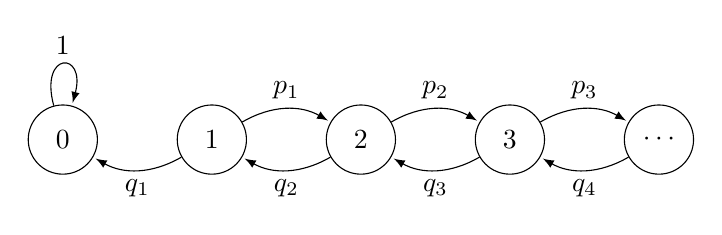
\begin{tikzpicture}

	\node[state] (0) {0};
	\node[state, right=of 0] (1) {1};
	\node[state, right=of 1] (2) {2};
	\node[state, right=of 2] (3) {3};
	\node[state, right=of 3] (4) {$\cdots$};

	\draw[every loop, >=latex]
	(0) edge[loop above] node {1} (0)
	(1) edge[bend left, above] node {$p_1$} (2)
	(2) edge[bend left, above] node {$p_2$} (3)
	(3) edge[bend left, above] node {$p_3$} (4)
	(1) edge[bend left, below] node {$q_1$} (0)
	(2) edge[bend left, below] node {$q_2$} (1)
	(3) edge[bend left, below] node {$q_3$} (2)
	(4) edge[bend left, below] node {$q_4$} (3);
	\end{tikzpicture}
	\end{center}

We would like to compute the probability of extinction $h_i = h_i^{\{0\}}$, starting from a population of size $i$. As always, $h$ is the minimal non-negative solution to
$$
h_0 = 1, \qquad h_i = p_i h_{i + 1} + q_i h_{i - 1} \text{ for } i \geq 1.
$$
This is \emph{not} a constant-coefficient difference equation, so we need to be slightly cleverer. Using $p_i + q_i = 1$, we can rearrange the relation into
$$
p_i (h_{i + 1} - h_i) = q_i (h_i - h_{i - 1}).
$$
So setting $u_i = h_{i - 1} - h_i$ (which will turn out to be non-negative), we get $u_{i + 1} = (q_i/p_i) u_i$, and iterating this down to $u_1$ gives
$$
u_{i + 1} = \left(\frac{q_i}{p_i}\right)\left(\frac{q_{i - 1}}{p_{i - 1}}\right) \cdots \left(\frac{q_1}{p_1}\right) u_1 = \gamma_i u_1, \quad \text{where } \gamma_i = \prod_{j = 1}^{i} \frac{q_j}{p_j},
$$
and we take $\gamma_0 = 1$ for convenience. Summing $u_j = h_{j - 1} - h_j$ over $j = 1, \dots, i$ telescopes to give
$$
h_i = 1 - u_1(\gamma_0 + \gamma_1 + \cdots + \gamma_{i - 1}).
$$
All that remains is to identify the constant $u_1$, and this is exactly what minimality is for. Everything hinges on whether the sum
$$
	\mathcal{S} = \sum_{i = 0}^{\infty} \gamma_i
$$
converges.

If $\mathcal{S} = \infty$, then any $u_1 > 0$ would make $h_i$ negative for large $i$, so we must have $u_1 = 0$, and $h_i = 1$ for all $i$ -- extinction is certain.

If $\mathcal{S} < \infty$, then to minimise $h_i$ we want $u_1$ as large as possible, subject to $h_i \geq 0$ for all $i$. Taking $i \rightarrow \infty$, the constraint becomes $1 - u_1 \mathcal{S} \geq 0$, so the minimal solution takes $u_1 = 1/\mathcal{S}$, giving
$$
h_i = \frac{\sum_{j = i}^{\infty} \gamma_j}{\sum_{j = 0}^{\infty} \gamma_j} < 1.
$$
So the population survives forever with positive probability exactly when $\sum \gamma_i$ converges, that is, when the birth rates outweigh the death rates sufficiently strongly.

\begin{example}[A Sanity Check]
	Let's check this against the gambler's ruin, where $p_i = p$ and $q_i = q$ are constant. Then $\gamma_i = (q/p)^i$, a geometric series, and $\mathcal{S} = \sum_i (q/p)^i$ converges if and only if $q < p$. If $q \geq p$ then $h_i = 1$, and if $q < p$ then
	$$
	h_i = \frac{\sum_{j = i}^{\infty}(q/p)^j}{\sum_{j = 0}^{\infty}(q/p)^j} = \left(\frac{q}{p}\right)^i,
	$$
	in agreement with what we found before. As a more interesting case, if the birth rate decays towards criticality like $p_i = \frac{1}{2} + \frac{c}{i}$ for a constant $c > 0$ (and large $i$), one can show $\gamma_i$ behaves like $i^{-4c}$, so extinction is uncertain if $c > 1/4$ and certain if $c \leq 1/4$ -- the boundary between the two behaviours is surprisingly delicate.
\end{example}

\subsection{Stopping Times and the Strong Markov Property}

We previously proved the \emph{simple Markov property}, that 
conditional on the value of a Markov chain at a given time $m$, the future is independent of the past.
This property required that we take some fixed time $m$ -- but what if $m$ itself is random? It's \emph{not} true in general\footnote{For example, let $T$ be the first time that a Markov chain hits some value $i$. Then if we condition on time $T - 1$, the future is then determined since the next step will be to $i$! You will see that this type of event is not allowed in our definition of stopping times.} that the Markov property still holds for an arbitrary random time, but it is true for certain kinds of times.

\begin{definition}[Stopping Times]
	A random time $T : \Omega \rightarrow \{0, 1, \dots\} \cup \{\infty\}$ is a \vocab{stopping time} for a Markov chain $X_n$ if for all $n \geq 0$ the event $\{T = n\}$ is given in terms of $X_0, X_1, \dots, X_n$ only.
\end{definition}

In particular, random times that `look into the future' are not stopping times. A straightforward example of a stopping time is the hitting time $T^A$ that we defined in the previous section.

\begin{example}[Stopping Times and Non-Stopping Times]
	Let $X_n$ track a gambler's fortune, and consider the following rules for when to leave the casino.
	\begin{enumerate}[label=(\roman*)]
		\item `Leave when your fortune first hits $\pounds 10$.' This is the hitting time $T_{\{10\}}$: the event $\{T_{\{10\}} = n\}$ is exactly $\{X_0 \neq 10, \dots, X_{n - 1} \neq 10, X_n = 10\}$, which depends only on $X_0, \dots, X_n$. So this is a stopping time -- it is a rule you could actually follow.
		\item `Leave one round after your fortune first hits $\pounds 10$.' This is $T_{\{10\}} + 1$, which is also a stopping time, as $\{T_{\{10\}} + 1 = n\}$ depends only on $X_0, \dots, X_{n - 1}$.
		\item `Leave one round \emph{before} your fortune first hits $\pounds 10$.' This is $T_{\{10\}} - 1$, and it is \emph{not} a stopping time: deciding whether to stop at time $n$ requires knowing $X_{n + 1}$. However appealing this rule sounds, there is no way to implement it.
	\end{enumerate}
\end{example}

With stopping times, we can indeed make a statement similar to the Markov property using random times.

\begin{theorem}[Strong Markov Property]	
Let $X_n$ be a Markov chain with transition matrix $P$, and let $T$ be a stopping time. Then conditional on $T < \infty$ and $X_T = i$, the sequence of random variables $(X_{T + n})_{n \geq 0}$ is $\markov(\delta_i, P)$ and is independent of $X_0, \dots, X_T$.
\end{theorem}
\begin{proof}
Let $H$ be an event given in terms of $X_0, \dots, X_{T - 1}$. Then it suffices to show that
\begin{align*}
	&\ \PP(X_{T + 1} = i_1, \dots, X_{T + n} = i_n, H \mid T < \infty, X_T = i)  \\
	&= \PP(X_1 = i_1, \dots, X_n = i_n \mid X_0 = i) \PP(H \mid T < \infty, X_T = i).
\end{align*}
The event $H \cap \{T = m\}$ is given in terms of $X_1, X_2, \dots, X_m$ only. Furthermore, $X_T = X_m$ when $T = m$. We condition on the event $H \cap \{T = m\} \cap \{X_m = i\}$ and use the simple Markov property at time $m$ to get
\begin{align*}
&\ \PP(X_{T + 1} = i_1, \dots, X_{T + n} = i_n, H \mid T < \infty, X_T = i) \\
&= \PP(X_1 = i_1, \dots, X_n = i_n) \PP(H, T = m, X_T = i).
\end{align*}
Summing this over $m = 0, 1, \dots$ and dividing by $\PP(T < \infty, X_T = i)$ then gives the desired result.
\end{proof}

The strong Markov property is one of those results whose usefulness is best appreciated by watching it in action. Let's return to our friend the gambler, and work out not just \emph{whether} they go bankrupt, but \emph{how long} it takes.

\begin{example}[Duration of the Gambler's Ruin]
	Consider again the gambler's ruin chain on $S = \{0, 1, 2, \dots\}$ with $P_{i, i + 1} = p$ and $P_{i, i - 1} = q = 1 - p$ for $i \geq 1$, and $0$ absorbing. Let $H = T_{\{0\}}$ be the time of bankruptcy, and suppose the gambler starts with $\pounds 1$.

	We are going to study the probability generating function
	$$
	G(s) = \EE[s^H \mid X_0 = 1] = \sum_{n = 0}^{\infty} s^n \, \PP(H = n \mid X_0 = 1), \quad \text{for } |s| < 1,
	$$
	where we adopt the convention $s^{\infty} = 0$ (recall it is possible that $H = \infty$).

	Conditioning on the first step, we have
	$$
	G(s) = p\EE[s^H \mid X_0 = 1, X_1 = 2] + q\EE[s^H \mid X_0 = 1, X_1 = 0].
	$$
	The second term is easy: if $X_1 = 0$ then $H = 1$, so $\EE[s^H \mid X_0 = 1, X_1 = 0] = s$. For the first term, starting from 2 the chain must pass through 1 on its way to 0, so we can write $H = 1 + H' + H''$, where $H'$ is the time taken to go from 2 to 1, and $H''$ is the time taken to go from 1 to 0 after that. The random time at which we first hit 1 is a stopping time, so by the strong Markov property $H'$ and $H''$ are independent, and each is distributed as $H$. Hence
	\begin{equation}
	G(s) = ps\, G(s)^2 + qs. \tag{$*$}
	\end{equation}
	Solving this quadratic in $G(s)$ gives
	$$
	G(s) = \frac{1 \pm \sqrt{1 - 4pqs^2}}{2ps}.
	$$
	We should be a little careful here -- a priori the sign might depend on $s$. But $G$ is a power series and hence continuous on $(0, 1)$, so a single sign must be taken throughout, and since $G(s)$ remains bounded as $s \downarrow 0$ we are forced to take the negative root:
	$$
	G(s) = \frac{1 - \sqrt{1 - 4pqs^2}}{2ps}.
	$$

	This function knows everything about the distribution of $H$. For example, the ruin probability is
	$$
	\PP(H < \infty \mid X_0 = 1) = \lim_{s \uparrow 1} G(s) = \frac{1 - \sqrt{1 - 4pq}}{2p} = \frac{1 - |p - q|}{2p} = \begin{cases}
		1 &\mbox{if } p \leq q, \\
		q/p &\mbox{if } p > q,
	   \end{cases}
	$$
	using $1 - 4pq = (p + q)^2 - 4pq = (p - q)^2$. This agrees (reassuringly!) with our hitting probability computation from before.

	We can also extract the mean. If $p \leq q$ then differentiating $(*)$ and rearranging gives
	$$
	G'(s) = \frac{pG(s)^2 + q}{1 - 2psG(s)},
	$$
	and letting $s \uparrow 1$ we obtain
	$$
	\EE[H \mid X_0 = 1] = \begin{cases}
		\frac{1}{q - p} &\mbox{if } p < q, \\
		\infty &\mbox{if } p = q = \frac{1}{2}.
	   \end{cases}
	$$
	So in a fair game, ruin is certain but takes infinite expected time -- exactly the curiosity we promised earlier.
\end{example}

\section{Recurrence and Transience}

\subsection{Recurrent and Transient States}

We now consider states that a Markov chain continues to come back to, or only visits finitely many times. It will turn out (perhaps surprisingly) that for each state, one of these two behaviours \emph{must} occur, in quite a strong sense: either the chain returns to the state infinitely often with probability 1, or it returns only finitely many times with probability 1. We give these two behaviours names.

\begin{definition}[Recurrence and Transience]
	Let $X_n$ be a Markov chain and let $i \in S$. We say the state $i$ is \vocab{recurrent} if
	$$
	\PP(X_n = i \text{ for infinitely many } n \mid X_0 = i) = 1,
	$$
	and we say $i$ is \vocab{transient} if
	$$
	\PP(X_n = i \text{ for infinitely many } n \mid X_0 = i) = 0.
	$$
\end{definition}

A priori, this probability could lie strictly between $0$ and $1$, in which case a state would be neither recurrent nor transient. The first goal of this section is to rule this out, and to obtain a usable criterion for telling the two cases apart. Doing this will be a lovely application of the strong Markov property.

We will need a little notation for `repeated visits'. Define the \vocab{first passage time} to a state $i \in S$ as
$$
T_i = \inf\{n \geq 1 \mid X_n = i\},
$$
which differs from the hitting time in that we do not count the chain as having returned to $i$ at time 0. More generally, we let $T_i^{(0)} = 0$ and inductively define the \vocab{$r$-th passage time} by
$$
T_i^{(r + 1)} = \inf\{n \geq T_i^{(r)} + 1 \mid X_n = i\},
$$
so that $T_i^{(1)} = T_i$. We also define the \vocab{return probability}
$$
f_i = \PP(T_i < \infty \mid X_0 = i),
$$
and the total \vocab{number of visits}
$$
V_i = \sum_{n = 0}^{\infty} \ii[X_n = i].
$$
With this notation, $i$ is recurrent exactly if $\PP(V_i = \infty \mid X_0 = i) = 1$, and transient exactly if this probability is 0.

Intuitively, every time the chain returns to $i$, it `starts afresh' by the strong Markov property, and so has probability $f_i$ of returning again. So the number of returns should behave like a run of independent trials each with success probability $f_i$. The following lemma makes this precise.

\begin{lemma}[Probability of Repeated Visits]
	Let $i \in S$. Then $\PP(V_i > r \mid X_0 = i) = f_i^r$, for all $r \in \N$.
\end{lemma}
\begin{proof}
	We use induction on $r$. For $r = 0$ the claim is clear, since if $X_0 = i$ then $V_i \geq 1$. Now note that, given $X_0 = i$, the event $\{V_i > r\}$ is precisely the event $\{T_i^{(r)} < \infty\}$. So suppose the result is true for $r$. Then
	\begin{align*}
		\PP(V_i > r + 1 \mid X_0 = i) &= \PP(T_i^{(r + 1)} < \infty \mid X_0 = i) \\
		&= \PP(T_i^{(r + 1)} < \infty, T_i^{(r)} < \infty \mid X_0 = i) \\
		&= \PP(T_i^{(r + 1)} < \infty \mid T_i^{(r)} < \infty, X_0 = i) \cdot \PP(T_i^{(r)} < \infty \mid X_0 = i) \\
		&= \PP(T_i^{(r + 1)} < \infty \mid T_i^{(r)} < \infty, X_0 = i) \cdot f_i^r.
	\end{align*}
	Now $T_i^{(r)}$ is a stopping time, and on the event $T_i^{(r)} < \infty$ we have $X_{T_i^{(r)}} = i$. So by the strong Markov property, conditional on $T_i^{(r)} < \infty$, the chain $(X_{T_i^{(r)} + n})_{n \geq 0}$ is $\markov(\delta_i, P)$, and hence
	$$
	\PP(T_i^{(r + 1)} < \infty \mid T_i^{(r)} < \infty, X_0 = i) = \PP(T_i < \infty \mid X_0 = i) = f_i,
	$$
	and thus $\PP(V_i > r + 1 \mid X_0 = i) = f_i^{r + 1}$, completing the induction.
\end{proof}

So given $X_0 = i$, the number of visits $V_i$ is a geometric random variable with parameter $1 - f_i$. In particular, if $f_i = 1$ then $V_i = \infty$ almost surely, and if $f_i < 1$ then $V_i$ is almost surely finite with finite expectation. This immediately gives us the dichotomy we were after.

\begin{theorem}[Recurrence and Transience Criterion]
	Let $X_n$ be a Markov chain with transition matrix $P$, and let $i \in S$. Then we have the following dichotomy:
	\begin{enumerate}[label=(\arabic*)]
		\item If $\PP(T_i< \infty \mid X_0 = i) = 1$, then $i$ is recurrent and $\sum_{n = 0}^{\infty} p_{i, i}(n)$ is infinite.
		\item If $\PP(T_i < \infty \mid X_0 = i) < 1$, then $i$ is transient and $\sum_{n = 0}^{\infty} p_{i, i}(n) < \infty$.
	\end{enumerate}
	In particular, every state is either recurrent or transient.
\end{theorem}
\begin{proof}
	Recall we can write $V_i$ using indicator functions as
	$
	V_i = \sum_{n = 0}^{\infty} \ii[X_n = i],
	$
	and then by linearity of expectation we can write
	$$
	\EE[V_i \mid X_0 = i] = \sum_{n = 0}^{\infty} \PP(X_n = i \mid X_0 = i) = \sum_{n = 0}^{\infty} p_{i, i}(n).
	$$

	\emph{Part (1)}. If $f_i = 1$, then for all $r$ we have $\PP(V_i > r \mid X_0 = i) = 1$, and thus $\PP(V_i = \infty \mid X_0 = i) = 1$, implying that $i$ is recurrent, and $\EE[V_i \mid X_0 = i] = \infty$, implying that $\sum_{n = 0}^{\infty} p_{i, i}(n) = \infty$.

	\emph{Part (2)}. If $f_i < 1$, then by the previous lemma we have $\EE[V_i \mid X_0 = i] = \sum_{r = 0}^{\infty} \PP(V_i > r \mid X_0 = i) = 1/(1 - f_i) < \infty$, implying that $\PP(V_i < \infty \mid X_0 = i) = 1$, so $i$ is transient, and $\sum_{n = 0}^{\infty} p_{i, i}(n) < \infty$.
\end{proof}

This criterion is genuinely useful -- the quantity $\sum_n p_{i,i}(n)$ is frequently something that we can estimate, and we will do exactly this when we study random walks on $\Z^d$ in the next section. But first, let's see how recurrence and transience interact with the class structure that we developed earlier. The headline is that recurrence and transience are \emph{class properties}: within a communicating class, all states behave in the same way.

\begin{theorem}[Recurrence and Transience of Communicating States]
	Let $x$ and $y$ be two states that communicate. Then either they are both recurrent or they are both transient.
\end{theorem}
\begin{proof}
	Suppose that $x$ is recurrent. We will show that $y$ is also recurrent. Since $x \rightarrow y$, there is some $m, l \in \N$ such that $p_{x, y}(m) > 0$ and $p_{y, x}(l) > 0$. Then we know that $\sum_{n = 0}^{\infty} p_{x, x}(n) = \infty$, and then
	\begin{align*}
	\sum_{n = 0}^{\infty} p_{y, y}(n) 
	&\geq \sum_{n = 0}^{\infty} 
	p_{y, y}(n + m + l) \\ 
	&\geq \sum_{n = 0}^{\infty} p_{y, x}(l) p_{x, x}(n) p_{x, y}(m)  \\
	&\geq p_{y, x}(l) p_{x, y}(m) \sum_{n = 0}^{\infty} p_{x, x}(n) = \infty,
	\end{align*}
	using the Chapman-Kolmogorov equations, and thus $y$ is recurrent by our criterion. The transient case follows since if $x$ was transient but $y$ was recurrent, then swapping the roles of $x$ and $y$ in the above argument would make $x$ recurrent, a contradiction.
\end{proof}

This immediately can be applied to the entire class structure of a Markov chain.

\begin{corollary}[Class Structure of Recurrence and Transience]
	Either all of the states in a communicating class are recurrent or they are all transient.
\end{corollary}

Recurrent communicating classes have a certain flavour to them, which should be intuitive. Really, for a communicating class to be recurrent we have to avoid getting stuck outside of that given communicating class. This forces closure of the communicating class.

\begin{theorem}[Closure of Recurrent Communicating Classes]
	If $C$ is a recurrent communicating class, then it must be closed.
\end{theorem}
\begin{proof}
	Suppose that $C$ was not closed. Then there exists $x \in C$ and $y \not \in C$ such that $x \rightarrow y$. Let $m$ be such that $p_{x, y}(m) > 0$. We first note that $y \not \rightarrow x$, since if we had $y \rightarrow x$ then $x$ and $y$ would communicate, and we would have $y \in C$. So if starting from $x$ we hit $y$ at some point, then we can never visit $x$ again. Thus
	$$
	\PP(V_x < \infty \mid X_0 = x) \geq \PP(X_m = y \mid X_0 = x) = p_{x, y}(m) > 0,
	$$
	so $x$ is not recurrent, which is a contradiction.
\end{proof}

In the other direction, a closed class need not be recurrent in general (we will meet examples of this when we study random walks), but it \emph{is} when the class is finite. This should feel right -- a chain trapped in a finite set of states has to visit some state infinitely often.

\begin{theorem}[Finite Closed Classes are Recurrent]
	A finite closed class is recurrent.
\end{theorem}
\begin{proof}
	Let $C$ be a finite closed class, and pick any state $x \in C$. Starting from $x$, the chain remains in $C$ forever (as $C$ is closed), and since $C$ is finite, there must be some state $y \in C$ that is visited infinitely often with positive probability, that is\footnote{This is really the pigeonhole principle: infinitely many time steps must be distributed amongst finitely many states, so if each $y \in C$ was visited infinitely often with probability zero, then with probability one every state would be visited finitely often -- which is impossible for a chain that stays in $C$ forever.},
	$$
	\PP(X_n = y \text{ for infinitely many } n \mid X_0 = x) > 0.
	$$
	Now, for the chain to visit $y$ infinitely often it must visit $y$ at least once, so conditioning on the first visit and applying the strong Markov property,
	\begin{align*}
		0 &< \PP(X_n = y \text{ for infinitely many } n \mid X_0 = x) \\
		&= \PP(T_y < \infty \mid X_0 = x) \cdot \PP(X_n = y \text{ for infinitely many } n \mid X_0 = y).
	\end{align*}
	In particular $\PP(X_n = y \text{ for infinitely many } n \mid X_0 = y) > 0$. But by the dichotomy this probability is either 0 or 1, so it equals 1, and $y$ is recurrent. Finally, since $x, y \in C$ they communicate, and recurrence is a class property, so all of $C$ is recurrent.
\end{proof}

\begin{corollary}[Finite Irreducible Chains are Recurrent]
	If $S$ is finite and $P$ is irreducible, then every state is recurrent.
\end{corollary}
\begin{proof}
	The whole state space is a single communicating class, which is certainly closed, and it is finite.
\end{proof}

So for \emph{finite} chains the story is pleasantly complete: the transient states are precisely those in non-closed classes, and the recurrent states are precisely those in closed classes. Let's see this classification on our worked example from the section on class structure.

\begin{example}[Classifying the States of a Finite Chain]
	Recall the five-state chain whose communicating classes we found to be $\{1, 2\}$ (closed), $\{3\}$ (not closed) and $\{4, 5\}$ (closed). By our theorems:
	\begin{itemize}
		\item The classes $\{1, 2\}$ and $\{4, 5\}$ are finite and closed, hence recurrent -- once the chain enters one of them, it revisits each of its states infinitely often.
		\item The class $\{3\}$ is not closed, hence not recurrent, so state 3 is transient. (Of course, we can also see this directly: on each visit to 3, the chain escapes forever with probability $2/3$, so the number of visits is geometric and finite.)
	\end{itemize}
	For an \emph{infinite} chain the classification is genuinely more subtle -- a closed class can be transient, as the asymmetric random walk on $\Z$ (which is irreducible, so its single class is closed) will shortly demonstrate.
\end{example}

Sometimes we don't need any of this machinery, because the return probability $f_i$ can simply be computed by hand. Here is an infinite chain where that happens.

\begin{example}[The Success-Runs Chain]
	Fix $p \in (0, 1)$ and $q = 1 - p$, and consider the chain on $S = \{0, 1, 2, \dots\}$ with
	$$
	P_{i, i + 1} = p, \qquad P_{i, 0} = q \quad \text{for all } i \geq 0.
	$$
	This chain tracks the length of the current run of successes in a sequence of independent trials: each success extends the run, and each failure resets the counter to zero. The chain is irreducible (we can reach $i$ from 0 via $i$ successes, and return in one failure).

	\begin{center}
	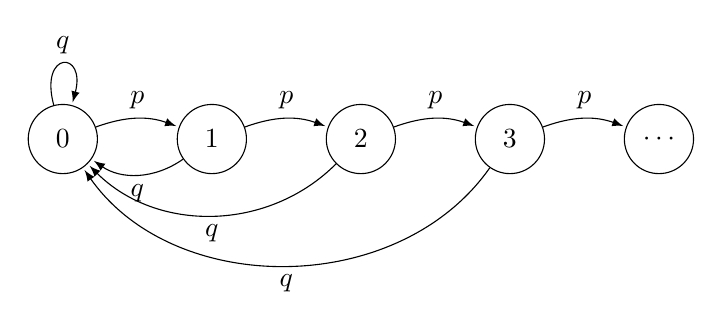
\begin{tikzpicture}

	\node[state] (0) {0};
	\node[state, right=of 0] (1) {1};
	\node[state, right=of 1] (2) {2};
	\node[state, right=of 2] (3) {3};
	\node[state, right=of 3] (4) {$\cdots$};

	\draw[every loop, >=latex]
	(0) edge[loop above] node {$q$} (0)
	(0) edge[bend left=20, auto=left] node {$p$} (1)
	(1) edge[bend left=20, auto=left] node {$p$} (2)
	(2) edge[bend left=20, auto=left] node {$p$} (3)
	(3) edge[bend left=20, auto=left] node {$p$} (4)
	(1) edge[bend left=35, below] node {$q$} (0)
	(2) edge[bend left=45, below] node {$q$} (0)
	(3) edge[bend left=55, below] node {$q$} (0);

	\end{tikzpicture}
	\end{center}

	Let's compute the return probability of state 0 directly. Starting from 0, the chain fails to return to 0 for $n$ consecutive steps precisely if the first $n$ trials are all successes, so
	$$
	\PP(T_0 > n \mid X_0 = 0) = p^n \rightarrow 0,
	$$
	giving $f_0 = \PP(T_0 < \infty \mid X_0 = 0) = 1$, so 0 is recurrent -- and hence, recurrence being a class property, the whole chain is recurrent. Moreover $T_0$ is geometrically distributed, with
	$$
	m_0 = \EE[T_0 \mid X_0 = 0] = \sum_{n = 0}^{\infty} \PP(T_0 > n \mid X_0 = 0) = \frac{1}{q} < \infty.
	$$
	So state 0 takes on average $1/q$ steps to revisit, however long the runs of successes may occasionally be. (Once we have developed the theory of invariant distributions, this will tell us instantly that $\pi_0 = q$ -- and it's a nice check that solving $\pi = \pi P$ gives the geometric distribution $\pi_i = qp^i$, whose value at 0 is indeed $q$.)
\end{example}

To close out this discussion, we prove one more result about irreducible, recurrent chains: not only does the chain return to where it started, it visits \emph{every} state with certainty, no matter where it begins.

\begin{theorem}[Recurrent Chains Visit Everything]
	Let $P$ be irreducible and recurrent. Then for all $x, y \in S$, $\PP(T_y < \infty \mid X_0 = x) = 1$.
\end{theorem}
\begin{proof}
	Fix $y \in S$, and let $m$ be such that $p_{y, x}(m) > 0$, which exists by irreducibility. Since $y$ is recurrent, using the simple Markov property at time $m$,
	\begin{align*}
		1 &= \PP(X_n = y \text{ for infinitely many } n \mid X_0 = y) \\
		&= \sum_{z \in S} \PP(X_m = z \mid X_0 = y) \, \PP(X_n = y \text{ for infinitely many } n \geq m \mid X_m = z) \\
		&= \sum_{z \in S} p_{y, z}(m) \, \PP(X_n = y \text{ for infinitely many } n \mid X_0 = z).
	\end{align*}
	Now each term $\PP(X_n = y \text{ for infinitely many } n \mid X_0 = z) \leq \PP(T_y < \infty \mid X_0 = z) \leq 1$, and the weights $p_{y, z}(m)$ sum to 1. So the only way the weighted average above can equal 1 is if
	$$
	\PP(T_y < \infty \mid X_0 = z) = 1 \quad \text{whenever } p_{y, z}(m) > 0.
	$$
	In particular, taking $z = x$ (recalling $p_{y,x}(m) > 0$) gives the result.
\end{proof}

\begin{aside}{Aside: A Generating Function Approach}
	There is a slick alternative route to the recurrence--transience dichotomy using generating functions, which is worth seeing. Fix a state $i$, write $f(n) = \PP(T_i = n \mid X_0 = i)$ for the distribution of the first return time, and consider the two generating functions
	$$
	F(s) = \sum_{n = 1}^{\infty} f(n)s^n, \qquad U(s) = \sum_{n = 0}^{\infty} p_{i, i}(n) s^n, \qquad |s| < 1.
	$$
	Conditioning on the time of the \emph{first} return to $i$, for $n \geq 1$ we have
	$$
	p_{i, i}(n) = \sum_{k = 1}^{n} f(k)\, p_{i, i}(n - k),
	$$
	using the strong Markov property at the first return time. But this is precisely a convolution! So multiplying by $s^n$ and summing over $n \geq 1$ (the $n = 0$ term of $U$ being 1),
	$$
	U(s) - 1 = F(s)U(s), \quad \text{that is,} \quad U(s) = \frac{1}{1 - F(s)}.
	$$
	Now we let $s \uparrow 1$. For power series with non-negative coefficients, we have $\lim_{s \uparrow 1} F(s) = \sum_n f(n) = f_i$ and $\lim_{s \uparrow 1} U(s) = \sum_n p_{i, i}(n)$, whether these are finite or infinite (this is \emph{Abel's lemma}, which follows from monotone convergence). Hence
	$$
	\sum_{n = 0}^{\infty} p_{i, i}(n) = \frac{1}{1 - f_i},
	$$
	with the convention $1/0 = \infty$. This identity contains the whole dichotomy at a glance: the left hand side is infinite if and only if $f_i = 1$. It also quantifies the relationship rather pleasingly -- for a transient state, the expected total number of visits is exactly $1/(1 - f_i)$, the mean of the geometric distribution we found earlier.

\end{aside}

\subsection{Random Walks on \texorpdfstring{$\Z^d$}{Zd} and Pólya's Theorem}

We now turn our attention to simple random walks in low and high dimensions, and in particular at an interesting result due to Pólya which informally says

\begin{center}
	{\color{blue} A drunk man will find his way home, but a drunk bird may get lost forever.}
\end{center}

Let's make this precise. The \vocab{simple random walk} on $\Z^d$ is the Markov chain with state space $\Z^d$ and transition probabilities
$$
P_{x, x + e_i} = P_{x, x - e_i} = \frac{1}{2d} \quad \text{for } i = 1, \dots, d,
$$
where $e_1, \dots, e_d$ are the standard basis vectors. That is, at each step the walker moves to one of its $2d$ neighbouring lattice points, chosen uniformly at random. For $d = 1$, this is a walk on the integers, moving left or right with probability $1/2$ each.

\begin{center}
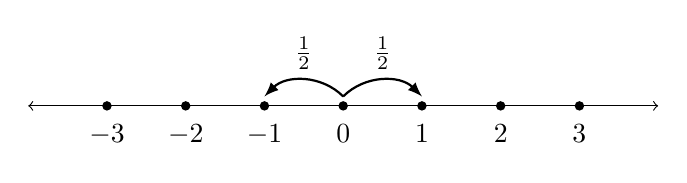
\begin{tikzpicture}
	\draw[<->] (-4, 0) -- (4, 0);
	\foreach \x in {-3,...,3} {
		\fill (\x, 0) circle (0.06);
		\node[below] at (\x, -0.12) {$\x$};
	}
	\draw[->, >=latex, thick] (0, 0.12) to[bend right=45] node[above] {$\frac{1}{2}$} (-1, 0.12);
	\draw[->, >=latex, thick] (0, 0.12) to[bend left=45] node[above] {$\frac{1}{2}$} (1, 0.12);
\end{tikzpicture}
\end{center}

The chain is clearly irreducible, so all states are of the same type -- either the walk is recurrent, and returns to its starting point over and over forever, or it is transient, and eventually escapes to infinity for good. Pólya's theorem tells us that which of these occurs depends only on the dimension.

\begin{theorem}[Pólya's Recurrence Theorem]
	The simple random walk on $\Z^d$ is recurrent for $d = 1$ and $d = 2$, and transient for $d \geq 3$.
\end{theorem}

The strategy for the proof is the one suggested by our recurrence and transience criterion: we will estimate the return probabilities $p_{0,0}(n)$, and determine whether $\sum_n p_{0, 0}(n)$ converges or diverges. The main analytic input is Stirling's formula, which we will not prove here.

\begin{fact}[Stirling's Formula]
	As $n \rightarrow \infty$, we have $n! \sim n^n e^{-n} \sqrt{2 \pi n}$, in the sense that the ratio of the two sides tends to 1.
\end{fact}

We take the three cases $d = 1, 2, 3$ in turn.

\begin{proof}[Proof ($d = 1$ is recurrent)]
	First note that the walk can only return to 0 at even times, since the parity of $X_n$ changes at every step. So it suffices to study $p_{0, 0}(2n)$.

	For the walk to be back at 0 after $2n$ steps, it must have taken exactly $n$ steps up and $n$ steps down. There are $\binom{2n}{n}$ ways to choose which steps are the `up' steps, and each arrangement occurs with probability $(1/2)^{2n}$. Hence
	$$
	p_{0, 0}(2n) = \binom{2n}{n} \left(\frac{1}{2}\right)^{2n} = \frac{(2n)!}{(n!)^2} \cdot \frac{1}{2^{2n}}.
	$$
	Applying Stirling's formula,
	$$
	p_{0, 0}(2n) \sim \frac{(2n)^{2n} e^{-2n}\sqrt{4 \pi n}}{n^{2n} e^{-2n} (2 \pi n)} \cdot \frac{1}{2^{2n}} = \frac{1}{\sqrt{\pi n}}.
	$$
	In particular, there is a constant $A > 0$ and some $n_0$ such that $p_{0, 0}(2n) \geq A/\sqrt{n}$ for all $n \geq n_0$. Thus
	$$
	\sum_{n = 0}^{\infty} p_{0, 0}(n) \geq \sum_{n \geq n_0} \frac{A}{\sqrt{n}} = \infty,
	$$
	and the walk is recurrent.
\end{proof}

\begin{remark}[Asymmetric Walks are Transient]
	Suppose instead the walk moves up with probability $p$ and down with probability $q = 1 - p$, where $p \neq q$. The same counting gives
	$$
	p_{0, 0}(2n) = \binom{2n}{n} (pq)^n \sim \frac{(4pq)^n}{\sqrt{\pi n}},
	$$
	and since $4pq < 1$ when $p \neq q$ (as $4pq = 1 - (p - q)^2$), the series $\sum_n p_{0,0}(n)$ converges by comparison with a geometric series. So \emph{any} asymmetry makes the walk transient -- the symmetric case is quite delicate!
\end{remark}

Now let's move up to two dimensions. The key idea here is a rather beautiful trick: if we rotate the lattice by $45\dg$, a simple random walk on $\Z^2$ splits into two \emph{independent} simple random walks on (scaled copies of) $\Z$.

\begin{center}
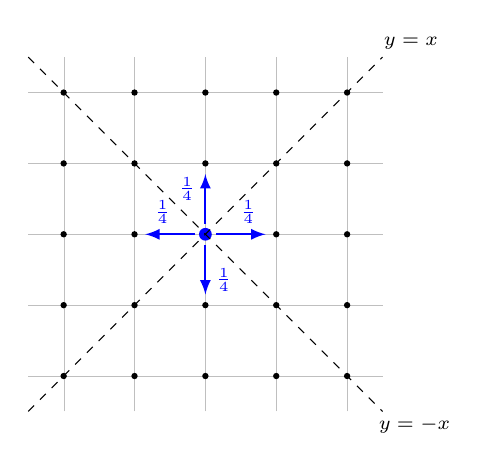
\begin{tikzpicture}[scale=0.9]
	\draw[ultra thin, color=lightgray] (-2.5, -2.5) grid (2.5, 2.5);
	\foreach \x in {-2,...,2}
		\foreach \y in {-2,...,2}
			\fill (\x, \y) circle (0.045);
	\fill[blue] (0, 0) circle (0.09);
	\draw[->, >=latex, thick, blue] (0.15, 0) -- (0.85, 0) node[pos=0.65, above] {\scriptsize $\frac{1}{4}$};
	\draw[->, >=latex, thick, blue] (-0.15, 0) -- (-0.85, 0) node[pos=0.65, above] {\scriptsize $\frac{1}{4}$};
	\draw[->, >=latex, thick, blue] (0, 0.15) -- (0, 0.85) node[pos=0.7, left] {\scriptsize $\frac{1}{4}$};
	\draw[->, >=latex, thick, blue] (0, -0.15) -- (0, -0.85) node[pos=0.7, right] {\scriptsize $\frac{1}{4}$};
	\draw[dashed] (-2.5, -2.5) -- (2.5, 2.5);
	\draw[dashed] (-2.5, 2.5) -- (2.5, -2.5);
	\node at (2.9, 2.7) {\scriptsize $y = x$};
	\node at (2.95, -2.7) {\scriptsize $y = -x$};
\end{tikzpicture}
\end{center}

\begin{proof}[Proof ($d = 2$ is recurrent)]
	Let $X_n$ be the simple random walk on $\Z^2$, and write $X_n = \xi_1 + \cdots + \xi_n$, where the steps $\xi_i$ are independent and uniform on the four unit vectors $\pm(1, 0)$ and $\pm(0, 1)$. We project onto the diagonal lines $y = x$ and $y = -x$, defining
	$$
	X_n^+ = \sum_{i = 1}^{n} \frac{\xi_i^{(1)} + \xi_i^{(2)}}{\sqrt{2}}, \qquad X_n^- = \sum_{i = 1}^{n} \frac{\xi_i^{(1)} - \xi_i^{(2)}}{\sqrt{2}},
	$$
	where $\xi_i = (\xi_i^{(1)}, \xi_i^{(2)})$.

	We claim that $X_n^+$ and $X_n^-$ are independent simple random walks on $\frac{1}{\sqrt{2}}\Z$. Indeed, checking each of the four possible values of $\xi_i$, we see that $(\xi_i^{(1)} + \xi_i^{(2)})/\sqrt{2}$ and $(\xi_i^{(1)} - \xi_i^{(2)})/\sqrt{2}$ each take the values $\pm 1/\sqrt{2}$ with probability $1/2$, and moreover each of the four possible combinations of signs occurs with probability $1/4$ -- so the two increments are independent. Since $X_n^+$ and $X_n^-$ are built from independent increments in this way, they are independent simple random walks, as claimed.

	Now, the walk $X_n$ is at the origin if and only if both projections are at 0. So using independence and our one-dimensional estimate,
	$$
	p_{0, 0}(2n) = \PP(X_{2n}^+ = 0)\,\PP(X_{2n}^- = 0) \sim \frac{1}{\sqrt{\pi n}} \cdot \frac{1}{\sqrt{\pi n}} = \frac{1}{\pi n}.
	$$
	Hence there is $A > 0$ with $p_{0, 0}(2n) \geq A/n$ for all sufficiently large $n$, and $\sum_n p_{0, 0}(n)$ diverges by comparison with the harmonic series. So the walk is recurrent.
\end{proof}

\begin{proof}[Proof ($d = 3$ is transient)]
	Again $p_{0, 0}(n) = 0$ for odd $n$, so we consider $p_{0, 0}(2n)$. For the walk to return to the origin after $2n$ steps, it must take $i$ steps in each of the $+x$ and $-x$ directions, $j$ steps in each of the $\pm y$ directions and $k$ steps in each of the $\pm z$ directions, for some $i + j + k = n$. Counting arrangements,
	\begin{align*}
	p_{0, 0}(2n) &= \sum_{\substack{i, j, k \geq 0 \\ i + j + k = n}} \frac{(2n)!}{(i!)^2 (j!)^2 (k!)^2} \left(\frac{1}{6}\right)^{2n} \\
	&= \binom{2n}{n} \left(\frac{1}{2}\right)^{2n} \sum_{\substack{i, j, k \geq 0 \\ i + j + k = n}} \left(\binom{n}{i, j, k} \left(\frac{1}{3}\right)^{n}\right)^2,
	\end{align*}
	where $\binom{n}{i, j, k} = \frac{n!}{i! j! k!}$ is the multinomial coefficient.

	Now, the numbers $\binom{n}{i, j, k} (1/3)^n$ are exactly the probabilities of the possible outcomes when placing $n$ balls into 3 boxes uniformly at random, so they sum to 1. Hence, bounding one factor in each square by the maximum,
	$$
	p_{0, 0}(2n) \leq \binom{2n}{n} \left(\frac{1}{2}\right)^{2n} \max_{i + j + k = n}\binom{n}{i, j, k} \left(\frac{1}{3}\right)^{n}.
	$$
	The multinomial coefficient is maximised when $i, j, k$ are as equal as possible\footnote{If, say, $i \geq j + 2$, then swapping $(i, j)$ for $(i - 1, j + 1)$ multiplies the coefficient by $i/(j + 1) > 1$.}, so writing $n = 3m$ we have
	$$
	p_{0, 0}(6m) \leq \binom{6m}{3m} \left(\tfrac{1}{2}\right)^{6m} \binom{3m}{m, m, m}\left(\tfrac{1}{3}\right)^{3m} \sim \frac{C}{m^{3/2}}
	$$
	for some constant $C$, applying Stirling's formula to each factorial. In particular, the sum $\sum_{m} p_{0, 0}(6m)$ converges.

	We are not quite done, since we have only summed over times divisible by 6. But the walk can always waste time by stepping out and back, so
	$$
	p_{0, 0}(6m) \geq \left(\frac{1}{6}\right)^2 p_{0, 0}(6m - 2) \quad \text{and} \quad p_{0, 0}(6m) \geq \left(\frac{1}{6}\right)^4 p_{0, 0}(6m - 4),
	$$
	which gives $p_{0, 0}(6m - 2) \leq 36\, p_{0, 0}(6m)$ and $p_{0, 0}(6m - 4) \leq 6^4\, p_{0, 0}(6m)$. Hence
	$$
	\sum_{n = 0}^{\infty} p_{0, 0}(2n) \leq (1 + 6^2 + 6^4)\sum_{m = 0}^{\infty} p_{0, 0}(6m) < \infty,
	$$
	and the walk is transient.
\end{proof}

\begin{remark}
	For $d > 3$, one can check that the first three coordinates of the simple random walk on $\Z^d$, observed at the times when one of them changes, form a simple random walk on $\Z^3$. If the walk on $\Z^d$ were recurrent, it would return to the origin infinitely often, forcing the embedded walk on $\Z^3$ to do the same -- contradicting transience in three dimensions. So the walk is transient for all $d \geq 3$.
\end{remark}

So the drunk man on the plane will stagger home eventually, but the drunk bird, with the extra dimension at its disposal, may drift away forever.

\section{Invariant Distributions}

\subsection{What is an Invariant Distribution?}

Having spent some time on the question of \emph{whether} a Markov chain comes back, we now turn to the long-run behaviour of the chain: if we let a Markov chain run for a very long time, what does its distribution look like?

Back when we computed $n$-step transition probabilities for the two-state chain, we found
$$
p_{1, 1}(n) = \frac{\beta}{\alpha+\beta}+\frac{\alpha}{\alpha+\beta} \cdot(1-\alpha-\beta)^{n},
$$
and if $\alpha + \beta < 2$ the second term dies away as $n \to \infty$, leaving $p_{1, 1}(n) \rightarrow \beta/(\alpha + \beta)$. The chain forgets where it started, and settles down to some limiting distribution. We would like to understand this phenomenon in general: when does a Markov chain settle down, and to what?

If the distribution of $X_n$ is to converge to something, a natural first step is to look for distributions that the chain leaves unchanged. Suppose $X_0$ has distribution $\pi$, and we would like $X_1$ to have distribution $\pi$ as well. Conditioning on the first state,
$$
\PP(X_1 = j) = \sum_{i \in S} \PP(X_0 = i)\PP(X_1 = j \mid X_0 = i) = \sum_{i \in S} \pi_i P_{i, j},
$$
so what we require is exactly that $\pi_j = \sum_{i} \pi_i P_{i, j}$ for all $j \in S$. Viewing $\pi$ as a row vector, this says precisely $\pi = \pi P$.

\begin{definition}[Invariant Distribution]
	A distribution\footnote{That is, $\pi = (\pi_i \mid i \in S)$ with $\pi_i \geq 0$ and $\sum_i \pi_i = 1$.} $\pi$ on $S$ is an \vocab{invariant distribution} (also called an \emph{equilibrium} or \emph{stationary} distribution) for the transition matrix $P$ if
	$$
	\pi = \pi P.
	$$
\end{definition}

In the language of linear algebra, $\pi$ is a left eigenvector of $P$ with eigenvalue 1, normalised to sum to 1. The name `invariant' is justified by the following observation.

\begin{proposition}[Invariance for All Time]
	Let $\pi$ be an invariant distribution for $P$, and let $X_n$ be $\markov(\pi, P)$. Then $X_n$ has distribution $\pi$ for all $n \geq 0$.
\end{proposition}
\begin{proof}
	The distribution of $X_n$ is given by the row vector $\pi P^n$, and by induction $\pi P^n = \pi P^{n - 1} = \cdots = \pi$.
\end{proof}

So a chain started in an invariant distribution is, in a distributional sense, in perfect equilibrium -- at every time it looks statistically identical. Let's compute an example.

\begin{example}[Invariant Distribution of the Two-State Chain]
	Consider our two-state chain with transition matrix
	$$
	P = \begin{pmatrix}
		1 - \alpha & \alpha \\
		\beta & 1 - \beta
	\end{pmatrix},
	$$
	with $\alpha, \beta \in (0, 1)$. To find an invariant distribution we solve $\pi = \pi P$, that is,
	\begin{align*}
		\pi_1 &= (1 - \alpha)\pi_1 + \beta \pi_2, \\
		\pi_2 &= \alpha \pi_1 + (1 - \beta) \pi_2.
	\end{align*}
	Both equations reduce to $\alpha \pi_1 = \beta \pi_2$, and combining this with $\pi_1 + \pi_2 = 1$ we get
	$$
	\pi = \left(\frac{\beta}{\alpha + \beta}, \frac{\alpha}{\alpha + \beta}\right).
	$$
	Notice that this is exactly the limit of $p_{1, 1}(n)$ and $p_{2, 1}(n)$ that we found by diagonalisation -- the limiting distribution of the chain is the invariant distribution. This is not a coincidence, as we will see in the next section.
\end{example}

\begin{example}[Invariant Distribution of a Three-State Chain]
	Recall the three-state chain with complex eigenvalues from Section 1, with transition matrix
	$$
	P = \begin{pmatrix}
		0 & 1 & 0 \\
		0 & 1/2 & 1/2 \\
		1/2 & 0 & 1/2
	\end{pmatrix}.
	$$
	Solving $\pi = \pi P$ coordinate by coordinate:
	\begin{align*}
		\pi_1 &= \tfrac{1}{2}\pi_3, \\
		\pi_2 &= \pi_1 + \tfrac{1}{2}\pi_2 \implies \pi_2 = 2\pi_1, \\
		\pi_3 &= \tfrac{1}{2}\pi_2 + \tfrac{1}{2}\pi_3 \implies \pi_3 = \pi_2.
	\end{align*}
	So $\pi \propto (1, 2, 2)$, and normalising gives $\pi = (1/5, 2/5, 2/5)$.

	Back in Section 1 we computed, with some effort involving complex eigenvalues,
	$$
	p_{1,1}(n) = \frac{1}{5} + \left(\frac{1}{2}\right)^n \left(\frac{4}{5}\cos\left(\frac{n \pi}{2}\right) - \frac{2}{5} \sin \left(\frac{n \pi}{2}\right)\right) \longrightarrow \frac{1}{5} = \pi_1,
	$$
	so the mysterious constant $1/5$ appearing there was the invariant probability of state 1 all along. The oscillating terms, damped by the factor $(1/2)^n = |\mu|^n$, describe \emph{how} the chain spirals in towards equilibrium.
\end{example}

The relationship between limits and invariant distributions goes both ways, at least when the state space is finite: if the $n$-step probabilities converge, then whatever they converge to must be invariant.

\begin{theorem}[Limits are Invariant]
	Let $S$ be finite, and suppose that for some $i \in S$ we have
	$
	p_{i, j}(n) \rightarrow \pi_j
	$
	as $n \rightarrow \infty$, for all $j \in S$. Then $\pi = (\pi_j \mid j \in S)$ is an invariant distribution.
\end{theorem}
\begin{proof}
	We first check that $\pi$ is a distribution. Certainly $\pi_j \geq 0$ for all $j$, and since $S$ is finite we may interchange the (finite) sum and the limit to get
	$$
	\sum_{j \in S} \pi_j = \sum_{j \in S}\lim_{n \to \infty} p_{i, j}(n) = \lim_{n \to \infty}\sum_{j \in S} p_{i, j}(n) = 1.
	$$
	Next we check invariance. Using the Chapman-Kolmogorov equations, and again exchanging the limit with the finite sum,
	$$
	\pi_j = \lim_{n \to \infty} p_{i, j}(n) = \lim_{n \to \infty}\sum_{k \in S} p_{i, k}(n - 1)P_{k, j} = \sum_{k \in S} \pi_k P_{k, j},
	$$
	so $\pi = \pi P$ as required.
\end{proof}

\begin{remark}
	Finiteness really is needed here, because exchanging limits with infinite sums is a dangerous business. For example, for the simple random walk on $\Z$ our estimates showed $p_{0, j}(n) \rightarrow 0$ for every $j$, and the zero vector is certainly not a probability distribution -- the mass of the walk `escapes to infinity' in the limit.
\end{remark}

This remark shows that invariant distributions need not exist in general. The next portion of this section is devoted to pinning down exactly when they do exist, and when they are unique. The answer will turn out to be a lovely story involving recurrence.

\subsection{Existence of Invariant Measures}

It will be convenient to temporarily drop the requirement that our distributions sum to 1. We say $\lambda = (\lambda_i \mid i \in S)$ is a \vocab{measure} on $S$ if $\lambda_i \geq 0$ for all $i$, and an \vocab{invariant measure} if additionally $\lambda = \lambda P$. If an invariant measure has finite total mass $\sum_i \lambda_i < \infty$, we can normalise it into an invariant distribution.

So where might an invariant measure come from? Here is a probabilistic way to think about it: fix a state $k$, and consider an `excursion' of the chain from $k$ back to $k$. If the chain is in equilibrium, then the amount of time it spends in each state $i$ per excursion ought to describe the equilibrium proportions. This motivates the following definition.

\begin{definition}[Expected Time Spent Per Excursion]
	Let $k \in S$. For each $i \in S$, define
	$$
	\nu_k(i) = \EE\left[\sum_{n = 0}^{T_k - 1} \ii[X_n = i] \;\middle|\; X_0 = k\right],
	$$
	the expected number of visits to $i$ during an excursion from $k$, before the chain first returns to $k$.
\end{definition}

Note that $\nu_k(k) = 1$, since the chain starts the excursion at $k$ and doesn't count its return. The following theorem says that this excursion recipe really does produce an invariant measure, at least when the chain is recurrent (so that excursions actually finish).

\begin{theorem}[Existence of Invariant Measures]
	Let $P$ be irreducible and recurrent. Then $\nu_k$ is an invariant measure, and moreover $0 < \nu_k(i) < \infty$ for all $i \in S$.
\end{theorem}
\begin{proof}
	Since $P$ is irreducible and recurrent, we know $T_k < \infty$ almost surely, and $X_{T_k} = k$. Because the excursion begins and ends at $k$, we can shift our time window by one step: counting visits to $i$ at times $0, 1, \dots, T_k - 1$ is the same as counting visits at times $1, 2, \dots, T_k$, since the only disagreement could be at the endpoints, where $X_0 = X_{T_k} = k$ contributes to both counts exactly when $i = k$. Hence, throughout taking probabilities conditional on $X_0 = k$,
	\begin{align*}
		\nu_k(i) &= \EE\left[\sum_{n = 1}^{T_k} \ii[X_n = i]\right] = \EE\left[\sum_{n = 1}^{\infty} \ii[X_n = i, T_k \geq n]\right] \\
		&= \sum_{n = 1}^{\infty} \PP(X_n = i, T_k \geq n) \\
		&= \sum_{n = 1}^{\infty} \sum_{j \in S} \PP(X_n = i \mid X_{n - 1} = j, T_k \geq n)\PP(X_{n - 1} = j, T_k \geq n).
	\end{align*}
	Now here is the key point: the event $\{T_k \geq n\} = \{T_k \leq n - 1\}^c$ is determined by $X_0, \dots, X_{n - 1}$ only, so by the simple Markov property $\PP(X_n = i \mid X_{n - 1} = j, T_k \geq n) = P_{j, i}$. Continuing,
	\begin{align*}
		\nu_k(i) &= \sum_{j \in S} P_{j, i} \sum_{n = 1}^{\infty} \PP(X_{n - 1} = j, T_k \geq n) \\
		&= \sum_{j \in S} P_{j, i}\, \EE\left[\sum_{n = 0}^{T_k - 1} \ii[X_n = j]\right] = \sum_{j \in S} \nu_k(j) P_{j, i},
	\end{align*}
	which is exactly the statement $\nu_k = \nu_k P$.

	It remains to show that $\nu_k$ is finite and positive. Note that invariance gives $\nu_k = \nu_k P^n$ for all $n$. Given $i \in S$, by irreducibility we can pick $n, m$ with $p_{k, i}(n) > 0$ and $p_{i, k}(m) > 0$. Then
	$$
	\nu_k(i) = \sum_{j \in S} \nu_k(j) p_{j, i}(n) \geq \nu_k(k)p_{k, i}(n) = p_{k, i}(n) > 0,
	$$
	and in the other direction
	$$
	1 = \nu_k(k) = \sum_{j \in S} \nu_k(j) p_{j, k}(m) \geq \nu_k(i)p_{i, k}(m),
	$$
	so $\nu_k(i) \leq 1/p_{i, k}(m) < \infty$.
\end{proof}

\subsection{Uniqueness of Invariant Measures}

We now know that irreducible recurrent chains have at least one invariant measure. Conveniently, it turns out they have essentially \emph{only} one -- every invariant measure is a scalar multiple of $\nu_k$.

\begin{theorem}[Uniqueness of Invariant Measures]
	Let $P$ be irreducible, and let $\lambda$ be an invariant measure with $\lambda_k = 1$. Then $\lambda \geq \nu_k$. If moreover $P$ is recurrent, then $\lambda = \nu_k$.
\end{theorem}
\begin{proof}
	For the first part, the idea is to repeatedly expand the invariance equation, each time splitting off the terms that pass through $k$. Indeed, for any $i$,
	$$
	\lambda_i = \sum_{j_1 \in S} \lambda_{j_1} P_{j_1, i} = P_{k, i} + \sum_{j_1 \neq k} \lambda_{j_1}P_{j_1, i},
	$$
	using $\lambda_k = 1$. Substituting the invariance equation into $\lambda_{j_1}$ again,
	$$
	\lambda_i = P_{k, i} + \sum_{j_1 \neq k} P_{k, j_1}P_{j_1, i} + \sum_{j_1, j_2 \neq k} \lambda_{j_2} P_{j_2, j_1}P_{j_1, i},
	$$
	and continuing in this way, after $n$ expansions we obtain
	\begin{align*}
	\lambda_i = P_{k, i} &+ \sum_{j_1 \neq k} P_{k, j_1}P_{j_1, i} + \cdots + \sum_{j_1, \dots, j_{n - 1} \neq k} P_{k, j_{n -1}} \cdots P_{j_2, j_1} P_{j_1, i} \\
	&+ \sum_{j_1, \dots, j_n \neq k} \lambda_{j_n} P_{j_n, j_{n - 1}} \cdots P_{j_1, i}.
	\end{align*}
	The final term is non-negative, and the earlier terms have a probabilistic meaning: the $m$-th term is exactly the probability that the chain started at $k$ is at $i$ at time $m$ without having returned to $k$ in between. That is,
	$$
	\lambda_i \geq \sum_{m = 1}^{n} \PP(X_m = i, T_k \geq m \mid X_0 = k),
	$$
	and letting $n \rightarrow \infty$, the right hand side converges\footnote{Here we are using the shifted-window description of $\nu_k(i)$ from the proof of the existence theorem: $\nu_k(i) = \sum_{m \geq 1} \PP(X_m = i, T_k \geq m \mid X_0 = k)$.} to $\nu_k(i)$. So $\lambda \geq \nu_k$.

	Now suppose $P$ is recurrent, so that $\nu_k$ is invariant by the previous theorem. Then $\mu = \lambda - \nu_k$ is also an invariant measure (it's non-negative by the first part), and $\mu_k = 1 - 1 = 0$. Given any $i \in S$, choose $n$ with $p_{i, k}(n) > 0$ by irreducibility. Then
	$$
	0 = \mu_k = \sum_{j \in S} \mu_j\, p_{j, k}(n) \geq \mu_i \, p_{i, k}(n),
	$$
	forcing $\mu_i = 0$. Hence $\lambda = \nu_k$.
\end{proof}

\subsection{Positive Recurrence and Existence of Invariant Distributions}

Let's take stock. For an irreducible recurrent chain, we have a family of invariant measures $\nu_k$ (one for each $k \in S$), all proportional to one another. To produce an invariant \emph{distribution} we need to normalise, which is possible exactly when $\nu_k$ has finite total mass. And the total mass has a beautiful interpretation:
$$
\sum_{i \in S} \nu_k(i) = \EE\left[\sum_{n = 0}^{T_k - 1} \sum_{i \in S}\ii[X_n = i] \;\middle|\; X_0 = k\right] = \EE\left[\sum_{n = 0}^{T_k - 1} 1 \;\middle|\; X_0 = k\right] = \EE[T_k \mid X_0 = k],
$$
the expected length of an excursion from $k$. So everything comes down to whether the \emph{mean return time} is finite. This suggests refining our notion of recurrence.

\begin{definition}[Positive and Null Recurrence]
	Let $i \in S$ be a recurrent state, and let $m_i = \EE[T_i \mid X_0 = i]$ denote the \vocab{mean return time} of $i$. We say $i$ is \vocab{positive recurrent} if $m_i < \infty$, and \vocab{null recurrent} if $m_i = \infty$.
\end{definition}

Note that a recurrent state has $T_i < \infty$ almost surely, but this does \emph{not} imply that $\EE[T_i] < \infty$ -- we saw exactly this phenomenon with the gambler's ruin. The following theorem ties everything in this section together.

\begin{theorem}[Existence and Uniqueness of Invariant Distributions]
	Let $P$ be irreducible. Then the following are equivalent:
	\begin{enumerate}[label=(\roman*)]
		\item every state is positive recurrent;
		\item some state is positive recurrent;
		\item $P$ has an invariant distribution $\pi$.
	\end{enumerate}
	Moreover, when these hold, the invariant distribution is unique and is given by
	$$
	\pi_i = \frac{1}{m_i} \quad \text{for all } i \in S.
	$$
\end{theorem}
\begin{proof}
	Clearly (i) implies (ii).

	\emph{(ii) implies (iii)}. Let $k$ be a positive recurrent state. Then $k$ is in particular recurrent, and since recurrence is a class property and $P$ is irreducible, $P$ is recurrent. So by our existence theorem, $\nu_k$ is an invariant measure, with total mass
	$
	\sum_i \nu_k(i) = m_k < \infty.
	$
	Hence
	$$
	\pi_i = \frac{\nu_k(i)}{m_k}
	$$
	defines an invariant distribution.

	\emph{(iii) implies (i)}. Suppose $\pi$ is an invariant distribution, and let $k \in S$ be any state; we will show $k$ is positive recurrent. First we claim $\pi_k > 0$: there is certainly some $i$ with $\pi_i > 0$, and choosing $n$ with $p_{i, k}(n) > 0$ by irreducibility, invariance gives
	$$
	\pi_k = \sum_{j \in S} \pi_j \, p_{j, k}(n) \geq \pi_i \, p_{i, k}(n) > 0.
	$$

	Before we can apply our uniqueness theorem, we need to know that $P$ is recurrent. Suppose instead that $P$ was transient. Then for all states $i, j$, we have $\sum_n p_{j, i}(n) < \infty$ and so certainly $p_{j, i}(n) \rightarrow 0$ as $n \to \infty$. But then, since $\pi_i = \sum_j \pi_j p_{j, i}(n)$ for every $n$, and the summands are dominated\footnote{We are using here the discrete version of the dominated convergence theorem: if $|f_n(j)| \leq g(j)$ with $\sum_j g(j) < \infty$ and $f_n(j) \rightarrow f(j)$ pointwise, then $\sum_j f_n(j) \rightarrow \sum_j f(j)$. In our case $\pi_j p_{j, i}(n) \leq \pi_j$, which is summable.} by the summable sequence $(\pi_j)$, we may pass to the limit and conclude $\pi_i = 0$ for all $i$ -- contradicting $\sum_i \pi_i = 1$. So $P$ is recurrent.

	Now define $\lambda_i = \pi_i / \pi_k$. This is an invariant measure with $\lambda_k = 1$, so by the uniqueness theorem, $\lambda = \nu_k$. Hence
	$$
	m_k = \sum_{i \in S} \nu_k(i) = \sum_{i \in S} \frac{\pi_i}{\pi_k} = \frac{1}{\pi_k} < \infty,
	$$
	so $k$ is positive recurrent, establishing (i). This computation also gives the final claim: $\pi_k = 1/m_k$ for every state $k$, and in particular the invariant distribution is unique, since its values are determined by the mean return times.
\end{proof}

This is a genuinely satisfying result: for irreducible chains, the existence of an invariant distribution is a sharp dividing line, and when it exists, the equilibrium probability of a state is exactly the reciprocal of its mean return time. States that the chain returns to quickly get lots of mass; states it takes ages to revisit get little.

\begin{example}[Mean Return Times of the Two-State Chain]
	For the two-state chain, the theorem predicts the mean return time
	$$
	m_1 = \frac{1}{\pi_1} = \frac{\alpha + \beta}{\beta},
	$$
	and this is easy enough to verify by hand -- always a healthy exercise. Starting from state 1, either the chain stays put (probability $1 - \alpha$), in which case $T_1 = 1$; or it jumps to state 2 (probability $\alpha$), where it must wait a $\operatorname{Geometric}(\beta)$ number of steps to jump back, giving $T_1 = 1 + \operatorname{Geometric}(\beta)$ in distribution. Hence
	$$
	m_1 = (1 - \alpha) \cdot 1 + \alpha \left(1 + \frac{1}{\beta}\right) = 1 + \frac{\alpha}{\beta} = \frac{\alpha + \beta}{\beta},
	$$
	exactly as predicted.
\end{example}

Before moving on, let's record one more consequence of the uniqueness theory, which gives the excursion counts $\nu_k$ a pleasingly simple form in the positive recurrent case.

\begin{corollary}[Visits Per Excursion]
	Let $P$ be irreducible with invariant distribution $\pi$. Then for any states $x, y \in S$, the expected number of visits to $y$ during an excursion from $x$ is
	$$
	\nu_x(y) = \frac{\pi_y}{\pi_x}.
	$$
\end{corollary}
\begin{proof}
	By the theorem above, $P$ is positive recurrent, and in particular recurrent, with $\pi_x > 0$ for all $x$. Now $\lambda_y = \pi_y / \pi_x$ defines an invariant measure with $\lambda_x = 1$, so by the uniqueness of invariant measures, $\lambda = \nu_x$.
\end{proof}

So, for example, between successive rainy days, the expected number of sunny days is simply the ratio of the equilibrium probabilities of sun and rain. Equilibrium ratios really do describe the fine structure of the chain's excursions, not just long-run averages.

Let's see the trichotomy of positive recurrence, null recurrence and transience play out on our favourite examples.

\begin{example}[The Simple Random Walk on $\Z$ is Null Recurrent]
	We proved via Pólya's theorem that the simple random walk on $\Z$ is recurrent. Is it positive recurrent? If it were, it would have an invariant distribution $\pi$. Solving $\pi = \pi P$ means
	$$
	\pi_i = \frac{1}{2}\pi_{i - 1} + \frac{1}{2}\pi_{i + 1} \quad \text{for all } i \in \Z,
	$$
	and we can spot the invariant measure $\lambda_i = 1$ for all $i$. By uniqueness of invariant measures (the walk is irreducible and recurrent), \emph{every} invariant measure is a constant multiple of this one -- and none of these have finite total mass, so no invariant distribution exists. Hence the walk is null recurrent: it always returns home, but the expected time to do so is infinite.
\end{example}

\begin{remark}
	One might hope for a converse: does having a `nice' invariant measure imply recurrence? No -- the simple random walk on $\Z^3$ is transient, and yet $\lambda_i = 1$ is a perfectly good invariant measure for it (the transition matrix is doubly stochastic). Existence of invariant \emph{measures} is cheap; it is invariant \emph{distributions} that carry real information.
\end{remark}

\begin{example}[A Transient Chain with Many Invariant Measures]
	Consider the asymmetric random walk on $\Z$ with $P_{i, i + 1} = p$, $P_{i, i - 1} = q$, where $p + q = 1$ and $p > q$. This chain is transient. Solving $\lambda = \lambda P$ gives the recurrence $\lambda_i = p\lambda_{i - 1} + q \lambda_{i + 1}$, with general solution
	$$
	\lambda_i = a + b \left(\frac{p}{q}\right)^i, \quad a, b \geq 0.
	$$
	These are genuinely different invariant measures (not multiples of each other), so the uniqueness theorem really does need recurrence. And again, none of them can be normalised, so there is no invariant distribution -- as must be the case, since the chain is not positive recurrent.
\end{example}

\begin{example}[A Positive Recurrent Walk]
	Now consider a random walk on $S = \{0, 1, 2, \dots\}$ with a drift towards the origin: let $0 < p < 1/2$, and set
	$$
	P_{i, i + 1} = p, \quad P_{i, i - 1} = q = 1 - p \quad \text{for } i \geq 1, \qquad P_{0, 1} = p, \quad P_{0, 0} = q.
	$$
	Rather than trying to compute mean return times directly, we look for an invariant distribution. The equations $\pi = \pi P$ read
	$$
	\pi_0 = q\pi_0 + q \pi_1, \qquad \pi_i = p\pi_{i - 1} + q\pi_{i + 1} \text{ for } i \geq 1.
	$$
	The first equation gives $\pi_1 = (p/q)\pi_0$, and then induction on the second\footnote{Substituting $\pi_i = (p/q)^i \pi_0$ into the second equation: $p (p/q)^{i-1} + q(p/q)^{i + 1} = (p/q)^i (q + p) = (p/q)^i$, as needed.} gives
	$$
	\pi_i = \left(\frac{p}{q}\right)^i \pi_0.
	$$
	Since $p < q$, this has finite total mass, and normalising gives the geometric distribution
	$$
	\pi_i = \left(1 - \frac{p}{q}\right)\left(\frac{p}{q}\right)^i.
	$$
	So by our theorem the chain is positive recurrent, with mean return times $m_i = 1/\pi_i$ -- and we found this out without ever computing an expectation directly. This is the invariant distribution machinery at its best.
\end{example}

\section{Convergence to Equilibrium}

We now come to the central limit-theorem-flavoured result of this course: for a nice enough Markov chain, the distribution of $X_n$ converges to the invariant distribution $\pi$, \emph{regardless of the initial distribution}. Run the chain for long enough and it forgets where it started.

\begin{center}
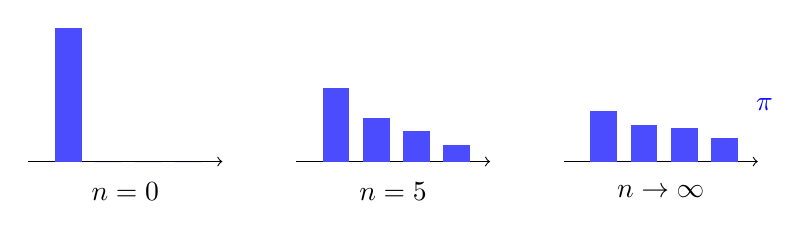
\begin{tikzpicture}[scale=0.85]
	% Panel 1: n = 0
	\begin{scope}[shift={(0,0)}]
		\draw[->] (-0.3, 0) -- (2.6, 0);
		\fill[blue!70] (0.1, 0) rectangle (0.5, 2.0);
		\fill[blue!70] (0.7, 0) rectangle (1.1, 0.0);
		\fill[blue!70] (1.3, 0) rectangle (1.7, 0.0);
		\fill[blue!70] (1.9, 0) rectangle (2.3, 0.0);
		\node at (1.15, -0.45) {$n = 0$};
	\end{scope}
	% Panel 2: n small
	\begin{scope}[shift={(4,0)}]
		\draw[->] (-0.3, 0) -- (2.6, 0);
		\fill[blue!70] (0.1, 0) rectangle (0.5, 1.1);
		\fill[blue!70] (0.7, 0) rectangle (1.1, 0.65);
		\fill[blue!70] (1.3, 0) rectangle (1.7, 0.45);
		\fill[blue!70] (1.9, 0) rectangle (2.3, 0.25);
		\node at (1.15, -0.45) {$n = 5$};
	\end{scope}
	% Panel 3: limit
	\begin{scope}[shift={(8,0)}]
		\draw[->] (-0.3, 0) -- (2.6, 0);
		\fill[blue!70] (0.1, 0) rectangle (0.5, 0.75);
		\fill[blue!70] (0.7, 0) rectangle (1.1, 0.55);
		\fill[blue!70] (1.3, 0) rectangle (1.7, 0.5);
		\fill[blue!70] (1.9, 0) rectangle (2.3, 0.35);
		\node at (1.15, -0.45) {$n \to \infty$};
		\node[blue] at (2.7, 0.85) {$\pi$};
	\end{scope}
\end{tikzpicture}
\end{center}

Of course, some hypotheses will be needed. We have already seen that we should assume irreducibility and positive recurrence, so that an invariant distribution exists and is unique. But there is one more, sneakier obstruction, which we address first.

\subsection{Aperiodicity}

Consider the Markov chain that cycles deterministically around three states, as below.

\begin{center}
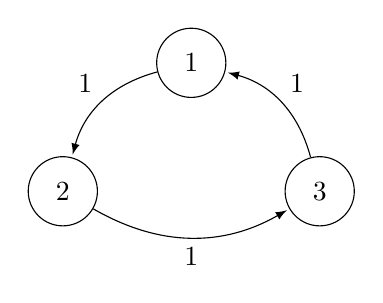
\begin{tikzpicture}

\node[state] (1) {1};
\node[state, below left=of 1] (2) {2};
\node[state, below right=of 1] (3) {3};

\draw[every loop, >=latex]
(1) edge[bend right, auto=right] node {$1$} (2)
(2) edge[bend right, auto=right] node {$1$} (3)
(3) edge[bend right, auto=right] node {$1$} (1);

\end{tikzpicture}
\end{center}

This chain is irreducible and positive recurrent, and its invariant distribution is the uniform one, $\pi = (1/3, 1/3, 1/3)$. But started from state 1, we have $\PP(X_n = 1) = 1$ when $3 \mid n$ and $\PP(X_n = 1) = 0$ otherwise -- the distribution of $X_n$ just cycles, and certainly doesn't converge to $\pi$. The chain never forgets its starting point, because its position modulo 3 remembers it forever. To rule out this kind of parity problem, we introduce the notion of periodicity.

\begin{definition}[Period]
	For a state $i \in S$, the \vocab{period} of $i$ is
	$$
	d_i = \gcd\{n \geq 1 \mid p_{i, i}(n) > 0\}.
	$$
	We say the state $i$ is \vocab{aperiodic} if $d_i = 1$.
\end{definition}

In the cycle above, each state has period 3. In the simple random walk on $\Z$, each state has period 2 -- and indeed we took care to work with $p_{0,0}(2n)$ throughout our analysis of it. More generally, the simple random walk on any \emph{bipartite} graph (one whose vertices can be 2-coloured so that every edge joins different colours) has period 2, since every closed walk has even length: the chain forever alternates between the two colour classes, and its colour at time $n$ remembers the parity of $n$. On the other hand, note that a single self-loop anywhere in an irreducible chain is enough to give that state period 1 (as $p_{i,i}(1) > 0$), and we shall see shortly that aperiodicity then spreads to every state.

For our purposes, the importance of aperiodicity is the following characterisation.

\begin{lemma}[Aperiodicity Criterion]
	A state $i$ is aperiodic if and only if $p_{i, i}(n) > 0$ for all sufficiently large $n$.
\end{lemma}
\begin{proof}
	Let $D = \{n \geq 1 \mid p_{i, i}(n) > 0\}$. One direction is easy: if $D$ contains all sufficiently large integers, then it certainly has greatest common divisor 1 (say, it contains two consecutive integers).

	For the other direction, first note that $D$ is closed under addition: if $a, b \in D$ then $p_{i, i}(a + b) \geq p_{i,i}(a) p_{i, i}(b) > 0$ by Chapman-Kolmogorov. Now suppose $\gcd D = 1$. Then there is some finite collection $n_1, \dots, n_r \in D$ with $\gcd\{n_1, \dots, n_r\} = 1$, and so by Bézout's lemma\footnote{Strictly, Bézout's lemma as usually stated handles two integers; the general case follows by induction on $r$.} there are integers $a_1, \dots, a_r$ with $a_1 n_1 + \cdots + a_r n_r = 1$. Collecting the positive and negative terms, we can write $M - N = 1$, where $M$ and $N$ are each non-negative integer combinations of the $n_s$, and hence (assuming $N \neq 0$; if $N = 0$ then $1 \in D$ and we're immediately done) both $M$ and $N$ lie in $D$ by closure under addition.

	So $D$ contains the consecutive integers $N$ and $N + 1$. Now take any $n \geq N^2$, and write $n = qN + s$ with $0 \leq s < N$. Then $q \geq N > s$, so
	$$
	n = (q - s)N + s(N + 1)
	$$
	expresses $n$ as a non-negative integer combination of $N$ and $N + 1$. Hence $n \in D$, and $D$ contains every integer at least $N^2$.
\end{proof}

Like recurrence and transience, aperiodicity turns out to be a class property, so for irreducible chains we can simply speak of \emph{the chain} being aperiodic.

\begin{lemma}[Aperiodicity is a Class Property]
	Suppose $P$ is irreducible and some state $i$ is aperiodic. Then every state is aperiodic.
\end{lemma}
\begin{proof}
	Let $j \in S$. By irreducibility there are $n, m$ with $p_{j, i}(n) > 0$ and $p_{i, j}(m) > 0$. Then for any $r$,
	$$
	p_{j, j}(n + r + m) \geq p_{j, i}(n) \, p_{i, i}(r) \, p_{i, j}(m),
	$$
	and by the previous lemma the middle factor is positive for all sufficiently large $r$. Hence $p_{j, j}(s) > 0$ for all sufficiently large $s$, and $j$ is aperiodic.
\end{proof}

\subsection{The Convergence Theorem}

We can now state and prove the main theorem of this section.

\begin{theorem}[Convergence to Equilibrium]
	Let $P$ be irreducible and aperiodic with invariant distribution $\pi$, and let $X_n$ be $\markov(\lambda, P)$ for any initial distribution $\lambda$. Then for all $j \in S$,
	$$
	\PP(X_n = j) \rightarrow \pi_j \quad \text{as } n \rightarrow \infty.
	$$
	In particular, taking $\lambda = \delta_i$, we have $p_{i, j}(n) \rightarrow \pi_j$ for all $i, j \in S$.
\end{theorem}

The proof uses a technique known as \emph{coupling}, which is worth dwelling on for a moment, as it's one of the loveliest ideas in probability. We want to compare the chain $X_n$ with a chain in equilibrium. So we simply run a second, independent copy $Y_n$ of the chain, started in the invariant distribution. The trick is then this: we watch the two chains until the (random) moment they happen to collide, and after that moment, we make $X$ `copy' $Y$. Copying $Y$ doesn't change the distribution of $X$ (by the strong Markov property, both chains restart identically from the collision point), but once they've collided, our chain literally \emph{is} in equilibrium. So all we need is that the collision happens eventually, and this is a recurrence statement, which we have the tools to prove.

\begin{proof}
	Let $Y_n$ be $\markov(\pi, P)$, independent of $X_n$.

	\emph{Step 1: the product chain.} Consider the process $W_n = (X_n, Y_n)$ on the state space $S \times S$. By independence, $W_n$ is a Markov chain with initial distribution $\mu_{(x, y)} = \lambda_x \pi_y$ and transition matrix
	$$
	\widetilde{P}_{(x, y), (x', y')} = P_{x, x'}P_{y, y'}.
	$$
	We claim $\widetilde{P}$ is irreducible. Given states $(x, y)$ and $(x', y')$, choose $\ell$ and $m$ with $p_{x, x'}(\ell) > 0$ and $p_{y, y'}(m) > 0$. For any $r \geq 0$, we have $p_{x, x'}(\ell + r) \geq p_{x, x'}(\ell)p_{x', x'}(r)$, which by aperiodicity is positive for all sufficiently large $r$; similarly $p_{y, y'}(m + r) > 0$ for all large $r$. So for sufficiently large $n$, both $p_{x, x'}(n)$ and $p_{y, y'}(n)$ are positive\footnote{This is where aperiodicity earns its keep: without it, $p_{x, x'}(n)$ and $p_{y, y'}(n)$ might only be positive on disjoint sets of times (consider the 3-cycle), and the product chain fails to be irreducible.}, and hence
	$
	\widetilde{P}_{(x, y), (x', y')}(n) = p_{x, x'}(n)p_{y, y'}(n) > 0.
	$

	Moreover, $\widetilde{P}$ has an invariant distribution $\widetilde{\pi}_{(x, y)} = \pi_x \pi_y$, as is easily checked using invariance of $\pi$ in each coordinate. So by our existence and uniqueness theorem, the product chain is positive recurrent, and in particular recurrent.

	\emph{Step 2: the coupling time.} Fix any state $a \in S$, and let
	$$
	T = \inf\{n \geq 1 \mid W_n = (a, a)\}
	$$
	be the first time the two chains simultaneously sit at $a$. Since the product chain is irreducible and recurrent, our `recurrent chains visit everything' theorem gives $\PP(T < \infty) = 1$.

	\emph{Step 3: the swap.} Now define
	$$
	Z_n = \begin{cases}
		X_n &\mbox{if } n < T, \\
		Y_n &\mbox{if } n \geq T.
	   \end{cases}
	$$
	We claim that $Z_n$ has the same distribution as $X_n$, i.e.\ that $Z$ is $\markov(\lambda, P)$. To see this, consider the swapped product process
	$$
	W_n' = \begin{cases}
		(X_n, Y_n) &\mbox{if } n < T, \\
		(Y_n, X_n) &\mbox{if } n \geq T.
	   \end{cases}
	$$
	The time $T$ is a stopping time for $W$, and $W_T = (a, a)$. By the strong Markov property, conditional on $T < \infty$, the process $(W_{T + n})_{n \geq 0}$ is $\markov(\delta_{(a, a)}, \widetilde{P})$, independent of $W_0, \dots, W_T$. But both the transition matrix $\widetilde{P}$ and the state $(a, a)$ are symmetric under swapping the two coordinates, so the coordinate-swapped process $((Y_{T + n}, X_{T + n}))_{n \geq 0}$ is \emph{also} $\markov(\delta_{(a, a)}, \widetilde{P})$, independent of the same past. Gluing this back onto the pre-$T$ process, we conclude that $W'$ is a Markov chain with the same initial distribution and transition matrix as $W$. In particular its first coordinate, which is exactly $Z$, is $\markov(\lambda, P)$ as claimed.

	\emph{Step 4: the conclusion.} Since $Y_0 \sim \pi$ and $\pi$ is invariant, $\PP(Y_n = j) = \pi_j$ for all $n$. Now for any $j \in S$,
	\begin{align*}
		|\PP(X_n = j) - \pi_j| &= |\PP(Z_n = j) - \PP(Y_n = j)| \\
		&= |\PP(X_n = j, n < T) + \PP(Y_n = j, n \geq T) \\
		&\qquad - \PP(Y_n = j, n < T) - \PP(Y_n = j, n \geq T)| \\
		&= |\PP(X_n = j, n < T) - \PP(Y_n = j, n < T)| \\
		&\leq \PP(T > n).
	\end{align*}
	Since $T$ is almost surely finite, $\PP(T > n) \rightarrow 0$ as $n \rightarrow \infty$, and we are done.
\end{proof}

It is worth appreciating how much of the theory we developed went into this proof: invariant distributions, positive recurrence, the classification of when invariant distributions exist, the strong Markov property, and aperiodicity all played essential roles.

\begin{example}[The Two-State Chain, One Last Time]
	The two-state chain with $\alpha, \beta \in (0, 1)$ is irreducible, and aperiodic since $p_{1, 1}(1) = 1 - \alpha > 0$. So the convergence theorem applies, and predicts
	$$
	p_{1, 1}(n) \rightarrow \pi_1 = \frac{\beta}{\alpha + \beta},
	$$
	which is precisely what our explicit formula
	$
	p_{1, 1}(n) = \frac{\beta}{\alpha + \beta} + \frac{\alpha}{\alpha + \beta}(1 - \alpha - \beta)^n
	$
	shows, since $|1 - \alpha - \beta| < 1$. It's pleasing to see the general theorem and the bare-hands computation agree -- and of course, the theorem's real value is for chains where no explicit formula is available.
\end{example}

\begin{example}[Convergence of the Reflected Biased Walk]
	Recall the walk on $\{0, 1, 2, \dots\}$ with $P_{i, i + 1} = p$ and $P_{i, i - 1} = q$ for $i \geq 1$, and $P_{0, 1} = p$, $P_{0, 0} = q$, where $p < 1/2 < q$. We showed it is positive recurrent with geometric invariant distribution $\pi_i = (1 - p/q)(p/q)^i$. The chain is aperiodic thanks to the lazy loop at 0 ($P_{0,0} = q > 0$), so the convergence theorem applies:
	$$
	\PP(X_n = i) \rightarrow \left(1 - \frac{p}{q}\right)\left(\frac{p}{q}\right)^i \quad \text{for every } i,
	$$
	no matter the initial distribution. Computing $p_{i, j}(n)$ explicitly for this chain would be thoroughly unpleasant -- yet its limit comes almost for free. Note the contrast with the unreflected walk on $\Z$: one boundary and a drift towards it are enough to change the walk from null recurrent (or transient) to positive recurrent.
\end{example}

\begin{remark}[The Lazy Chain Trick]
	Periodicity, while a genuine obstruction to convergence, is a rather fragile one. Given any irreducible chain $P$, consider the \emph{lazy chain} $P' = \frac{1}{2}(I + P)$, which at each step flips a fair coin and either stays put or takes a step of $P$. Then $P'$ is aperiodic (each state has $P'_{i,i} \geq 1/2 > 0$), it is irreducible, and it has exactly the same invariant distributions as $P$, since $\pi P' = \frac{1}{2}\pi + \frac{1}{2}\pi P = \pi$ if and only if $\pi P = \pi$. So laziness destroys periodicity while preserving equilibrium -- a trick worth remembering.
\end{remark}

\begin{aside}{Aside: How Many Shuffles Suffice?}
	Convergence to equilibrium is not just an abstract limit theorem -- it is the mathematics of \emph{shuffling cards}. The arrangements of a deck of 52 cards form a set $S$ of size $52!$, and a shuffling method (repeatedly cutting and riffling, say) defines a Markov chain on $S$: the next arrangement depends only on the current one and the randomness of the shuffle. Provided the shuffle is `random enough' for the chain to be irreducible and aperiodic, our convergence theorem promises that the distribution of the deck's arrangement converges to the unique invariant distribution -- which, by the symmetry of the situation, is uniform on all $52!$ arrangements\footnote{A little more precisely: each shuffle composes the current arrangement with a random permutation, so the transition matrix satisfies $P_{\sigma, \tau} = P_{\rho\sigma, \rho\tau}$ for any permutation $\rho$, which forces each column of $P$ to sum to 1 as well as each row. For such \emph{doubly stochastic} matrices, the uniform distribution is invariant, since $\sum_{\sigma} \frac{1}{52!} P_{\sigma, \tau} = \frac{1}{52!}$.}. In other words, shuffle for long enough and the deck genuinely becomes perfectly mixed, regardless of how it started.

	The really interesting question -- \emph{how fast?} -- is beyond this course, but has a famously crisp answer: Bayer and Diaconis showed that for riffle shuffles of a 52-card deck, about \emph{seven} shuffles are needed before the distribution is close to uniform, with a sharp `cut-off' from poorly-mixed to well-mixed occurring around that point. The study of such mixing times is a thriving area of modern probability, and it all rests on the framework we have just built.

\end{aside}

\subsection{What Happens Without Positive Recurrence?}

If the chain is irreducible but \emph{not} positive recurrent, then there is no invariant distribution to converge to, and indeed the distribution of the chain flattens out entirely.

\begin{theorem}[Null Recurrent and Transient Chains Forget Everything]
	Let $P$ be irreducible and aperiodic, and suppose $P$ is not positive recurrent (that is, it is null recurrent or transient). Then for all $x, y \in S$,
	$$
	p_{x, y}(n) \rightarrow 0 \quad \text{as } n \rightarrow \infty.
	$$
\end{theorem}
\begin{proof}
	As in the convergence theorem, form the product chain on $S \times S$ with transition matrix $\widetilde{P}_{(x, y), (x', y')} = P_{x, x'}P_{y, y'}$, which is irreducible by aperiodicity (this part of the earlier proof did not use positive recurrence). We consider two cases.

	\emph{Case 1: $\widetilde{P}$ is transient.} For a transient chain, the expected total number of visits to any fixed state is finite from any starting point\footnote{Indeed, by the strong Markov property, the number of visits to state $w'$ starting from $w$ is bounded by a geometric random variable: $\EE[V_{w'} \mid W_0 = w] = \PP(T_{w'} < \infty \mid W_0 = w)/(1 - f_{w'}) < \infty$.}. Applying this to the product chain started at $(x, x)$, looking at visits to $(y, y)$,
	$$
	\sum_{n = 0}^{\infty} \widetilde{p}_{(x,x), (y,y)}(n) = \sum_{n = 0}^{\infty} p_{x, y}(n)^2 < \infty,
	$$
	so $p_{x, y}(n)^2 \rightarrow 0$, giving the result.

	\emph{Case 2: $\widetilde{P}$ is recurrent.} Note that in this case $P$ itself must be recurrent (if the product chain returns to $(y, y)$ infinitely often, its first coordinate returns to $y$ infinitely often), and hence $P$ is null recurrent, and the invariant measure $\nu_y$ (for any fixed $y \in S$) has infinite total mass $\sum_z \nu_y(z) = m_y = \infty$.

	Let $M > 0$. Since $\nu_y$ has infinite mass but is finite on each state, we can choose a \emph{finite} set $A \subseteq S$ with $\nu_y(A) = \sum_{z \in A}\nu_y(z) > M$. Define a distribution $\mu$ by
	$$
	\mu_z = \frac{\nu_y(z)}{\nu_y(A)} \ii[z \in A].
	$$
	The point of this construction is the following bound: for any $z \in S$ and $n \geq 0$, since $\mu \leq \nu_y / \nu_y(A)$ entrywise and $\nu_y$ is invariant,
	$$
	(\mu P^n)_z \leq \frac{(\nu_y P^n)_z}{\nu_y(A)} = \frac{\nu_y(z)}{\nu_y(A)}.
	$$
	In particular $(\mu P^n)_y \leq \nu_y(y)/\nu_y(A) = 1/\nu_y(A) < 1/M$.

	Now we couple. Let $(X_n, Y_n)$ be the product chain with initial distribution $\mu \times \delta_x$, that is, $X_0 \sim \mu$ and $Y_0 = x$ independently. Fix $s \in S$ and let $T = \inf\{n \geq 1 \mid (X_n, Y_n) = (s, s)\}$; since the product chain is irreducible and recurrent, $T < \infty$ almost surely. Defining $Z_n$ to follow $X$ before $T$ and $Y$ afterwards, exactly as in the convergence theorem, $Z$ is $\markov(\mu, P)$, so $\PP(Z_n = y) = (\mu P^n)_y < 1/M$. Then
	\begin{align*}
	p_{x, y}(n) = \PP(Y_n = y) &\leq \PP(Y_n = y, n \geq T) + \PP(T > n) \\
	&= \PP(Z_n = y, n \geq T) + \PP(T > n) \leq \frac{1}{M} + \PP(T > n).
	\end{align*}
	Taking $n \to \infty$ gives $\limsup_n p_{x, y}(n) \leq 1/M$, and since $M$ was arbitrary, $p_{x, y}(n) \rightarrow 0$.
\end{proof}

\begin{example}
	For the simple random walk on $\Z$ (null recurrent, though periodic -- consider instead its lazy version to meet the aperiodicity hypothesis) we can see this flattening concretely: our Stirling estimate gave
	$$
	p_{0, 0}(2n) \sim \frac{1}{\sqrt{\pi n}} \rightarrow 0.
	$$
	The walk keeps coming back to 0 forever, but the \emph{probability} of finding it at 0 (or any fixed state) at a given large time dwindles to nothing, as the walk spreads out over an ever-larger range of $\Z$.
\end{example}

\section{The Ergodic Theorem}

The convergence theorem tells us about the distribution of the chain at a single large time $n$. In this section we will prove a different kind of limit theorem, about the behaviour of a single realisation of the chain over time: the \emph{long-run proportion of time} spent in each state. This is the Markov chain analogue of the strong law of large numbers -- and indeed the strong law is exactly what we will use to prove it. Let us recall the statement (it is proved in a course on probability theory, and we will treat it as a black box).

\begin{fact}[Strong Law of Large Numbers]
	Let $U_1, U_2, \dots$ be independent, identically distributed, non-negative random variables with $\EE[U_1] = \mu \leq \infty$. Then
	$$
	\PP\left(\frac{U_1 + \cdots + U_r}{r} \rightarrow \mu \text{ as } r \rightarrow \infty\right) = 1.
	$$
	This holds also when $\mu = \infty$, in the sense that the averages tend to infinity almost surely.
\end{fact}

We will apply this to the durations of the successive excursions of a Markov chain from a state. Since these excursions are independent (thanks to the strong Markov property), the total time taken for $r$ excursions grows like $r \cdot m_i$, and inverting this relationship will give us the proportion of time spent at $i$. Let's set up notation: define the \vocab{number of visits to $i$ before time $n$} as
$$
V_i(n) = \sum_{m = 0}^{n - 1} \ii[X_m = i],
$$
so that $V_i(n)/n$ is the proportion of the first $n$ time steps spent at $i$.

\begin{theorem}[Ergodic Theorem]
	Let $P$ be irreducible, and let $X_n$ be $\markov(\lambda, P)$ for any initial distribution $\lambda$. Then
	$$
	\PP\left(\frac{V_i(n)}{n} \rightarrow \frac{1}{m_i} \text{ as } n \rightarrow \infty \right) = 1,
	$$
	where $m_i = \EE[T_i \mid X_0 = i]$ is the mean return time, and we interpret $1/\infty = 0$. In particular, if $P$ is positive recurrent with invariant distribution $\pi$, then the long-run proportion of time spent in each state $i$ is almost surely $\pi_i$.
\end{theorem}

Note the hypotheses: there is no aperiodicity assumption here, and the result holds even in the null recurrent and transient cases. Time averages are more forgiving than distributional limits. To see the contrast at its starkest, consider our deterministic 3-cycle: the distribution of $X_n$ cycles forever and never converges, but the proportion of time spent in each state converges beautifully to $1/3 = 1/m_i$, as each state is visited exactly once every three steps.

\begin{proof}
	First suppose $P$ is transient. Then the total number of visits $V_i = \lim_n V_i(n)$ is almost surely finite, so
	$$
	\frac{V_i(n)}{n} \leq \frac{V_i}{n} \rightarrow 0,
	$$
	and since transient states have $\PP(T_i < \infty \mid X_0 = i) < 1$, certainly $m_i = \infty$ and $1/m_i = 0$, in agreement.

	So suppose $P$ is recurrent, and fix the state $i$. Let $T = T_i$ be the first passage time to $i$. By our `recurrent chains visit everything' theorem, $T < \infty$ almost surely, and by the strong Markov property the process $(X_{T + n})_{n \geq 0}$ is $\markov(\delta_i, P)$. Moreover, discarding the initial segment of the chain before time $T$ changes neither the limit of $V_i(n)/n$ (we discard only finitely many steps) nor $1/m_i$. So it suffices to prove the result when $\lambda = \delta_i$, i.e.\ assuming $X_0 = i$.

	Now let $U_r = T_i^{(r)} - T_i^{(r - 1)}$ be the length of the $r$-th excursion from $i$. By the strong Markov property applied at the stopping times $T_i^{(r - 1)}$ (which are finite almost surely, by recurrence), the excursion lengths $U_1, U_2, \dots$ are independent and identically distributed with mean $\EE[U_1] = m_i$. Writing $T_i^{(r)} = U_1 + \cdots + U_r$, the strong law of large numbers gives
	$$
	\frac{T_i^{(r)}}{r} \rightarrow m_i \quad \text{almost surely}
	$$
	(including in the null recurrent case $m_i = \infty$).

	The final step is to relate the passage times back to $V_i(n)$, which we do by a sandwiching argument. Since $X_0 = i$, at time $n - 1$ the chain has made exactly $V_i(n)$ visits to $i$ (counting the one at time 0), so the $(V_i(n) - 1)$-th return has happened by time $n - 1$, but the $V_i(n)$-th has not:
	$$
	T_i^{(V_i(n) - 1)} \leq n - 1 < T_i^{(V_i(n))}.
	$$
	Dividing through by $V_i(n)$,
	$$
	\frac{T_i^{(V_i(n) - 1)}}{V_i(n) - 1} \cdot \frac{V_i(n) - 1}{V_i(n)} \leq \frac{n}{V_i(n)} \leq \frac{T_i^{(V_i(n))}}{V_i(n)}.
	$$
	By recurrence $V_i(n) \rightarrow \infty$ almost surely, so both the left and right hand sides converge almost surely to $m_i$ (using our strong law statement along the random subsequence $r = V_i(n)$, which is valid since $V_i(n) \rightarrow \infty$). Hence $n / V_i(n) \rightarrow m_i$ almost surely, which is exactly the claim.

	Finally, if $P$ is positive recurrent, then $\pi_i = 1/m_i$ by our existence and uniqueness theorem.
\end{proof}

\begin{remark}
	The ergodic theorem is the theoretical justification for estimating $\pi$ by \emph{simulation}: run the chain for a long time and record the empirical proportions of time spent in each state. This idea underlies Markov chain Monte Carlo, one of the most widely used computational techniques in modern statistics -- there, one cleverly \emph{constructs} a Markov chain whose invariant distribution is a distribution one wishes to sample from. (The construction is usually done via detailed balance, which we discuss next.)
\end{remark}

\begin{example}[An Unreliable Printer]
	A printer is either working or broken, and its state is inspected each morning. If it is working today, it breaks down overnight with probability $\alpha$; if it is broken, an engineer manages to fix it overnight with probability $\beta$. This is exactly our two-state chain, with invariant distribution
	$$
	\pi = \left(\frac{\beta}{\alpha + \beta}, \frac{\alpha}{\alpha + \beta}\right)
	$$
	on the states $\{\text{working}, \text{broken}\}$. By the ergodic theorem, the long-run \emph{proportion of days} on which the printer works is, with probability one,
	$$
	\frac{V_{\text{working}}(n)}{n} \rightarrow \frac{\beta}{\alpha + \beta}.
	$$
	Note the subtle upgrade from the convergence theorem: not only is the printer working with probability close to $\beta/(\alpha + \beta)$ on any particular distant day, but the actual observed fraction of good days converges to this value on almost every realisation of history. If, say, each working day generates income $c$, then the long-run income rate is $c\beta/(\alpha + \beta)$ per day, almost surely -- statements of this form are exactly what the ergodic theorem is for.
\end{example}

\section{Time Reversal}

\subsection{Reversing a Markov Chain}

Here is a curious question to end the course with: if we film a Markov chain in equilibrium and play the tape backwards, what do we see? The Markov property is symmetric in time to a greater extent than one might expect -- conditional on the present, the past and future are independent, and this description doesn't distinguish a direction of time. Indeed, it turns out the reversed film shows another Markov chain, and we can say exactly which one.

\begin{theorem}[Time Reversal]
	Let $P$ be irreducible with invariant distribution $\pi$, and let $X_n$ be $\markov(\pi, P)$. Fix $N \geq 1$, and define $Y_n = X_{N - n}$ for $0 \leq n \leq N$. Then $(Y_n)_{0 \leq n \leq N}$ is $\markov(\pi, \widehat{P})$, where
	$$
	\widehat{P}_{i, j} = \frac{\pi_j}{\pi_i} P_{j, i}.
	$$
	Moreover $\widehat{P}$ is also irreducible, with invariant distribution $\pi$.
\end{theorem}

The chain $\widehat{P}$ is called the \vocab{time reversal} of $P$. (Note $\pi_i > 0$ for all $i$ by irreducibility and positive recurrence, so there are no division-by-zero worries here.)

\begin{proof}
	First, $\widehat{P}$ is a genuine (stochastic) transition matrix: its entries are non-negative, and using $\pi = \pi P$,
	$$
	\sum_{j \in S} \widehat{P}_{i, j} = \frac{1}{\pi_i}\sum_{j \in S} \pi_j P_{j, i} = \frac{\pi_i}{\pi_i} = 1.
	$$

	Next we check that $Y$ has the right finite-dimensional distributions. For any states $i_0, \dots, i_N$,
	\begin{align*}
		\PP(Y_0 = i_0, \dots, Y_N = i_N) &= \PP(X_0 = i_N, X_1 = i_{N -1}, \dots, X_N = i_0) \\
		&= \pi_{i_N} P_{i_N, i_{N - 1}} \cdots P_{i_1, i_0}.
	\end{align*}
	Now we repeatedly substitute using $\pi_j P_{j, i} = \pi_i \widehat{P}_{i, j}$, moving from left to right: first $\pi_{i_N}P_{i_N, i_{N -1}} = \pi_{i_{N - 1}}\widehat{P}_{i_{N - 1}, i_N}$, then combining $\pi_{i_{N-1}}$ with the next factor, and so on. After $N$ substitutions we obtain
	$$
	\PP(Y_0 = i_0, \dots, Y_N = i_N) = \pi_{i_0}\widehat{P}_{i_0, i_1} \cdots \widehat{P}_{i_{N - 1}, i_N},
	$$
	which by our very first theorem (the probability of a sequence of states) says exactly that $Y$ is $\markov(\pi, \widehat{P})$.

	For invariance of $\pi$ under $\widehat{P}$,
	$$
	\sum_{i \in S} \pi_i \widehat{P}_{i, j} = \sum_{i \in S} \pi_j P_{j, i} = \pi_j.
	$$
	Finally, for irreducibility, let $i, j \in S$. By irreducibility of $P$ there is a path $i = i_0, i_1, \dots, i_k = j$ with $P_{i_0, i_1}P_{i_1, i_2} \cdots P_{i_{k - 1}, i_k} > 0$. Then, reversing the path,
	$$
	\widehat{P}_{i_k, i_{k -1}}\cdots \widehat{P}_{i_1, i_0} = \frac{\pi_{i_0}}{\pi_{i_k}} P_{i_0, i_1} \cdots P_{i_{k - 1}, i_k} > 0,
	$$
	(the intermediate $\pi$ factors telescope), so $j \rightarrow i$ in the reversed chain, as required.
\end{proof}

\begin{remark}
	The hypothesis that the chain starts \emph{in equilibrium} is doing real work here. If $X_0$ had some other distribution, the reversed process would generally fail to be a homogeneous Markov chain at all -- for instance, if $X_0 = i$ is deterministic, then watching the film backwards, the process is mysteriously compelled to arrive at state $i$ at the final frame, which no homogeneous transition mechanism can arrange. Equilibrium is exactly the condition that makes the chain look statistically the same at every time, so that reversing time doesn't distinguish any particular moment.
\end{remark}

\begin{example}[Reversing a Biased Cycle]
	Let $n \geq 3$ and consider the walk on $\Z_n$ (the integers modulo $n$) that steps clockwise with probability $2/3$ and anticlockwise with probability $1/3$. By symmetry, the invariant distribution is uniform, $\pi_i = 1/n$. The time reversal is then
	$$
	\widehat{P}_{i, j} = \frac{\pi_j}{\pi_i}P_{j, i} = P_{j, i},
	$$
	so $\widehat{P}_{i, i - 1} = P_{i - 1, i} = 2/3$ and $\widehat{P}_{i, i + 1} = 1/3$: the reversed chain is the walk biased \emph{anticlockwise} instead. This is exactly what intuition demands -- a film of a clockwise-drifting walker, played backwards, shows an anticlockwise-drifting walker. In particular $\widehat{P} \neq P$ here, and the direction of drift is precisely the feature that betrays the direction of time.
\end{example}

\subsection{Detailed Balance and Reversibility}

The most interesting case of time reversal is when running the film backwards is \emph{undetectable} -- when the reversed chain is statistically identical to the original.

\begin{definition}[Reversibility]
	Let $P$ be irreducible with invariant distribution $\pi$. The chain is \vocab{reversible} (in equilibrium) if $\widehat{P} = P$, that is, if
	$$
	\pi_i P_{i, j} = \pi_j P_{j, i} \quad \text{for all } i, j \in S.
	$$
	These equations are called the \vocab{detailed balance equations}.
\end{definition}

The detailed balance equations have a very physical interpretation. In equilibrium, the quantity $\pi_i P_{i, j}$ is the probability of seeing the chain make the specific transition $i \rightarrow j$ at a given time step -- a `flow of probability' from $i$ to $j$. Invariance ($\pi = \pi P$) says that the total flow into each state balances the total flow out. Detailed balance is a much stronger, local statement: the flow from $i$ to $j$ equals the flow from $j$ to $i$, \emph{along every edge individually}.

\begin{center}
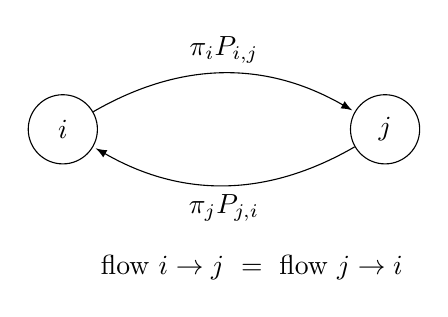
\begin{tikzpicture}

\node[state] (1) {$i$};
\node[state, right=3.2cm of 1] (2) {$j$};

\draw[every loop, >=latex]
(1) edge[bend left, auto=left] node {$\pi_i P_{i, j}$} (2)
(2) edge[bend left, auto=left] node {$\pi_j P_{j, i}$} (1);

\node at (2.4, -1.75) {flow $i \to j$ \;=\; flow $j \to i$};

\end{tikzpicture}
\end{center}

Why do we care? One excellent practical reason:

\begin{lemma}[Detailed Balance Implies Invariance]
	Let $P$ be a transition matrix and $\mu$ a distribution satisfying the detailed balance equations $\mu_i P_{i, j} = \mu_j P_{j, i}$ for all $i, j$. Then $\mu$ is an invariant distribution for $P$.
\end{lemma}
\begin{proof}
	We simply sum:
	$$
	(\mu P)_j = \sum_{i \in S} \mu_i P_{i, j} = \sum_{i \in S} \mu_j P_{j, i} = \mu_j. \qedhere
	$$
\end{proof}

The detailed balance equations are a system of `one equation per pair of states', each involving only two unknowns, and are usually \emph{far} easier to solve than $\pi = \pi P$. So a sensible strategy when hunting for an invariant distribution is: try detailed balance first. If it has a solution, you've found $\pi$ (and shown the chain is reversible as a bonus). If not, the chain isn't reversible, and you must go back to $\pi = \pi P$.

\begin{example}[A Chain That is Not Reversible]
	Let $n \geq 3$, and consider the random walk on $\Z_n$ (the integers modulo $n$) which steps clockwise with probability $2/3$ and anticlockwise with probability $1/3$:
	$$
	P_{i, i + 1} = \frac{2}{3}, \quad P_{i, i - 1} = \frac{1}{3} \quad \text{(indices mod } n).
	$$
	By symmetry we can check that $\pi_i = 1/n$ is invariant: each state receives flow $\frac{1}{n}\cdot\frac{2}{3}$ from its anticlockwise neighbour, and $\frac{1}{n} \cdot \frac{1}{3}$ from its clockwise neighbour, totalling $1/n$. But detailed balance fails:
	$$
	\pi_i P_{i, i + 1} = \frac{2}{3n} \neq \frac{1}{3n} = \pi_{i + 1}P_{i + 1, i}.
	$$
	And this makes perfect sense -- in equilibrium there is a net current of probability flowing clockwise around the cycle, and if we watched a film of this chain we could tell whether it was being played backwards, by watching which way the walker predominantly moves.
\end{example}

\begin{example}[A Reversible Chain]
	Now cut the cycle open: consider the same walk on $\{0, 1, \dots, n - 1\}$, but where the walk cannot wrap around, say
	$$
	P_{i, i + 1} = \frac{2}{3} \;\; (i < n - 1), \quad P_{i, i - 1} = \frac{1}{3} \;\; (i > 0), \quad P_{0, 0} = \frac{1}{3}, \quad P_{n - 1, n - 1} = \frac{2}{3}.
	$$
	This time there is nowhere for a net current to circulate, and indeed detailed balance succeeds: the equations
	$$
	\pi_i P_{i, i + 1} = \pi_{i + 1}P_{i + 1, i} \implies \pi_{i + 1} = 2\pi_i,
	$$
	give $\pi_i = c \cdot 2^i$, and normalising, $\pi_i = 2^i / (2^n - 1)$. So this chain is reversible, with an invariant distribution that piles up geometrically at the right-hand end.
\end{example}

The moral of the pair of examples: reversibility is characteristically obstructed by \emph{cycles with a preferred direction}. On tree-like or line-like state spaces, where every transition must eventually be retraced, chains tend to be reversible. In fact, for chains on the non-negative integers that only ever step to a neighbour, this is a theorem.

\begin{proposition}[Birth-Death Chains are Reversible]
	Let $P$ be an irreducible birth-death chain on $S = \{0, 1, 2, \dots\}$ (or a finite interval of integers), i.e.\ $P_{i, j} = 0$ whenever $|i - j| > 1$, and suppose $P$ has an invariant distribution $\pi$. Then the chain is reversible.
\end{proposition}
\begin{proof}
	We must show $\pi_i P_{i, j} = \pi_j P_{j, i}$ for all $i, j$. This is trivial if $i = j$ or $|i - j| > 1$, so it suffices to show $\pi_i P_{i, i + 1} = \pi_{i + 1}P_{i + 1, i}$ for all $i$, and we induct on $i$. Consider the invariance equation at state 0. Since only states 0 and 1 can move to 0,
	$$
	\pi_0 = \pi_0 P_{0, 0} + \pi_1 P_{1, 0},
	$$
	and $P_{0, 0} = 1 - P_{0, 1}$, so rearranging gives $\pi_0 P_{0, 1} = \pi_1 P_{1, 0}$, the base case. For the inductive step, invariance at state $i + 1$ reads
	$$
	\pi_{i + 1} = \pi_i P_{i, i + 1} + \pi_{i + 1}P_{i + 1, i + 1} + \pi_{i + 2}P_{i + 2, i + 1},
	$$
	and substituting $P_{i + 1, i + 1} = 1 - P_{i + 1, i} - P_{i + 1, i + 2}$ along with the inductive hypothesis $\pi_i P_{i, i + 1} = \pi_{i + 1}P_{i + 1, i}$, everything cancels down to
	$$
	\pi_{i + 1}P_{i + 1, i + 2} = \pi_{i + 2}P_{i + 2, i + 1},
	$$
	completing the induction.
\end{proof}

So the Ehrenfest urn didn't just \emph{happen} to satisfy detailed balance -- any chain with that skeleton must. The probabilistic explanation is the one we gave above: to travel from $i$ to $j$ the chain must cross each intermediate edge, and every crossing of an edge in one direction must (in the long run) be matched by a crossing in the other direction, since the chain cannot go round any other way.

Let's do one more substantial example, which is a classical model from statistical physics.

\begin{example}[The Ehrenfest Urn]
	Two chambers are connected by a small hole, and contain $N$ gas molecules between them. At each time step, a molecule is chosen uniformly at random and moves through the hole to the other chamber. Let $X_n$ be the number of molecules in the left chamber, so $X_n$ is a Markov chain on $\{0, 1, \dots, N\}$ with
	$$
	P_{i, i - 1} = \frac{i}{N}, \qquad P_{i, i + 1} = \frac{N - i}{N}.
	$$
	For example, when $N = 3$ the chain looks as follows.
	\begin{center}
	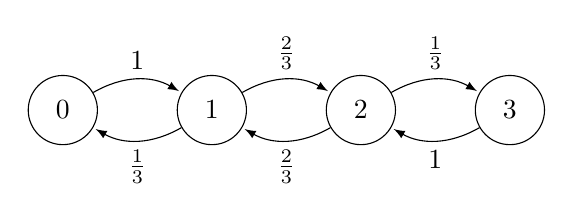
\begin{tikzpicture}

	\node[state] (0) {0};
	\node[state, right=of 0] (1) {1};
	\node[state, right=of 1] (2) {2};
	\node[state, right=of 2] (3) {3};

	\draw[every loop, >=latex]
	(0) edge[bend left, above] node {$1$} (1)
	(1) edge[bend left, above] node {$\frac{2}{3}$} (2)
	(2) edge[bend left, above] node {$\frac{1}{3}$} (3)
	(1) edge[bend left, below] node {$\frac{1}{3}$} (0)
	(2) edge[bend left, below] node {$\frac{2}{3}$} (1)
	(3) edge[bend left, below] node {$1$} (2);

	\end{tikzpicture}
	\end{center}
	The state space is line-like, so we optimistically try detailed balance:
	$$
	\pi_i P_{i, i + 1} = \pi_{i + 1}P_{i + 1, i} \implies \pi_{i + 1} = \pi_i \cdot \frac{N - i}{i + 1}.
	$$
	Iterating this down to $\pi_0$ gives
	$$
	\pi_i = \pi_0 \cdot \frac{N (N - 1) \cdots (N - i + 1)}{i!} = \pi_0 \binom{N}{i},
	$$
	and since $\sum_i \binom{N}{i} = 2^N$, normalising gives
	$$
	\pi_i = \binom{N}{i} \frac{1}{2^N}.
	$$
	So in equilibrium, the number of molecules in the left chamber is distributed as $\operatorname{Bin}(N, 1/2)$ -- exactly as if each molecule independently tossed a fair coin to choose its chamber. The chain is reversible: watching the molecules shuffle back and forth, we cannot tell which way time is flowing.

	The mean return times contain a famous lesson. The mean return time to a half-full chamber is
	$$
	m_{N/2} = \frac{1}{\pi_{N/2}} = \frac{2^N}{\binom{N}{N/2}} \approx \sqrt{\frac{\pi N}{2}},
	$$
	(taking $N$ even, and using Stirling), which is tiny. But the mean return time to the state where the left chamber is \emph{empty} is
	$$
	m_0 = \frac{1}{\pi_0} = 2^N,
	$$
	which for $N$ of the order of Avogadro's number is unimaginably vast. So the chain \emph{is} recurrent -- all the air in the room will eventually gather in one half of it! -- but the expected time for this is so astronomically long that we will never observe it. This resolves (or at least, quantifies) the apparent conflict between microscopic reversibility and the macroscopic arrow of time.
\end{example}

\subsection{Random Walks on Graphs}

We finish with a family of Markov chains where detailed balance works beautifully: random walks on graphs. Let $G = (V, E)$ be a finite connected graph. The \vocab{simple random walk on $G$} is the Markov chain with state space $V$ in which, at each step, the walker moves to a uniformly random neighbour of its current vertex. Writing $d(v)$ for the degree of the vertex $v$, the transition matrix is
$$
P_{u, v} = \begin{cases}
	\frac{1}{d(u)} &\mbox{if } uv \in E, \\
	0 &\mbox{otherwise}.
   \end{cases}
$$
Connectedness of $G$ makes the chain irreducible. So, what is the invariant distribution? Following our own advice, we try detailed balance first. For an edge $uv \in E$, the equations read
$$
\pi_u \cdot \frac{1}{d(u)} = \pi_v \cdot \frac{1}{d(v)},
$$
which says exactly that $\pi_v \propto d(v)$. Since $\sum_{v} d(v) = 2|E|$ (each edge is counted from both ends), normalising gives the following.

\begin{proposition}[Invariant Distribution for Random Walk on a Graph]
	The simple random walk on a finite connected graph $G = (V, E)$ is reversible, with invariant distribution
	$$
	\pi_v = \frac{d(v)}{2|E|}, \quad v \in V.
	$$
\end{proposition}

In equilibrium, the walker is found at each vertex with probability proportional to its degree -- well-connected vertices are visited more. A special case worth noting: if $G$ is \emph{regular} (all degrees equal), the invariant distribution is uniform. So a random walk on the vertices of a cube, or on a cycle, spends its time equally amongst all vertices in the long run -- and, for instance, a walker on the corners of a cube takes on average $m_v = 1/\pi_v = 8$ steps to return to its starting corner.

Let's see the general case on a concrete graph.

\begin{example}[A Walk on a Small Graph]
	Consider the simple random walk on the graph below, where each vertex is labelled with its invariant probability $\pi_v = d(v)/2|E|$; here $|E| = 6$, so $2|E| = 12$.
	\begin{center}
	\begin{tikzpicture}[scale=1.4]
		\draw[thick] (0, 1.2) -- (1.2, 1.2) -- (1.2, 0) -- (0, 0) -- cycle;
		\draw[thick] (0, 1.2) -- (1.2, 0);
		\draw[thick] (1.2, 0) -- (2.3, 0);
		\fill[blue] (0, 1.2) circle (0.05) node[black, above left] {$a$: $\tfrac{3}{12}$};
		\fill[blue] (1.2, 1.2) circle (0.05) node[black, above right] {$b$: $\tfrac{2}{12}$};
		\fill[blue] (1.2, 0) circle (0.05) node[black, below left] {$c$: $\tfrac{4}{12}$};
		\fill[blue] (0, 0) circle (0.05) node[black, below left] {$d$: $\tfrac{2}{12}$};
		\fill[blue] (2.3, 0) circle (0.05) node[black, below right] {$e$: $\tfrac{1}{12}$};
	\end{tikzpicture}
	\end{center}
	The vertex $c$, with its four edges, carries the most mass, while the pendant vertex $e$ carries the least. By our earlier theory, we can immediately read off facts that would be quite painful to compute directly: for example the mean return time to $e$ is $m_e = 1/\pi_e = 12$, while the mean return time to $c$ is $m_c = 12/4 = 3$.
\end{example}

\begin{aside}{Aside: The Random Surfer}
	A relative of the random walk on a graph powers one of the most consequential algorithms ever deployed: Google's \emph{PageRank}. Imagine a `random surfer' on the web, who at each step clicks a uniformly random link on their current page -- a random walk on the (directed!) graph of the web. The importance of a page is then defined to be its invariant probability $\pi_v$: the long-run proportion of time the surfer spends there, which by the ergodic theorem is a genuinely meaningful quantity. A page is important if many important pages link to it, and this apparently circular definition is resolved exactly by the equation $\pi = \pi P$.

	Because the web graph is directed, the lovely formula $\pi_v \propto d(v)$ no longer applies (detailed balance fails -- links very much have a preferred direction), and the chain is far from irreducible. The fix is a version of the lazy chain trick: with small probability at each step, the surfer teleports to a uniformly random page. This makes the chain irreducible and aperiodic, so a unique invariant distribution exists and can be found by simply iterating $\lambda \mapsto \lambda P$ -- which, by convergence to equilibrium, approaches $\pi$ from any starting guess.

\end{aside}

\begin{example}[The Knight on a Chessboard]
	As a parting example: place a knight on the corner square of an otherwise empty chessboard, and let it make uniformly random legal moves. How long, on average, until it first returns to its starting corner?

	This looks like a nightmare of a computation, but the theory makes it almost trivial. The knight performs a simple random walk on the graph whose vertices are the 64 squares, with edges given by legal knight moves. This graph is connected, so
	$$
	m_{\text{corner}} = \frac{1}{\pi_{\text{corner}}} = \frac{2|E|}{d(\text{corner})} = \frac{\sum_v d(v)}{d(\text{corner})}.
	$$
	Summing the degrees over the whole board\footnote{The degrees form the pattern: corner squares have 2 moves, squares adjacent to corners have 3 or 4, central squares have 8, and so on; carrying out the count gives $\sum_v d(v) = 336$.} gives $336$, and a corner square has exactly 2 knight moves, so
	$$
	m_{\text{corner}} = \frac{336}{2} = 168.
	$$
	A lovely answer, obtained with essentially no computation -- a fitting note on which to end the course.
\end{example}

\section*{Epilogue: The Big Picture}

This is a good point to pause and assemble the whole story in one place. For an \emph{irreducible} Markov chain, everything we have proved organises the possible behaviours into a clean trichotomy.

\begin{itemize}
	\item \emph{Transient.} The chain visits each state only finitely often, and escapes to infinity: $\PP(T_i < \infty \mid X_0 = i) < 1$ and $\sum_n p_{i,i}(n) < \infty$. There is no invariant distribution, and $p_{i, j}(n) \rightarrow 0$. The long-run proportion of time in each state is 0. (Example: the simple random walk on $\Z^3$.)
	\item \emph{Null recurrent.} The chain returns to each state infinitely often, but with infinite mean return time. Invariant \emph{measures} exist and are unique up to scaling, but have infinite mass, so there is still no invariant \emph{distribution}; again $p_{i, j}(n) \rightarrow 0$ (given aperiodicity) and the long-run proportions are 0. The chain is recurrent but only just. (Example: the simple random walk on $\Z$ or $\Z^2$.)
	\item \emph{Positive recurrent.} Mean return times are finite, and there is a unique invariant distribution $\pi$, given by $\pi_i = 1/m_i$. The long-run proportion of time spent in state $i$ is $\pi_i$ almost surely (the ergodic theorem, no aperiodicity needed), and if the chain is additionally aperiodic then $\PP(X_n = i) \rightarrow \pi_i$ from any initial distribution (convergence to equilibrium). (Examples: every finite irreducible chain, and drifting walks like the reflected biased walk.)
\end{itemize}

For finite state spaces, only the third behaviour is possible for irreducible chains, which is why finite chains are so pleasant: an invariant distribution always exists, and irreducibility plus aperiodicity guarantees convergence to it.

Finally, the theory of time reversal gives a practical route to finding $\pi$: solve the detailed balance equations if you can (as for birth-death chains, the Ehrenfest urn, and random walks on graphs), and fall back on $\pi = \pi P$ when the chain carries a genuine probability current around a cycle. With these tools, remarkably many questions -- mean return times, long-run proportions, limiting probabilities -- reduce to a small amount of linear algebra.

Of course, this is only the beginning of the story of Markov processes. Natural next steps include chains that evolve in \emph{continuous} time (the subject of the Part II course `Applied Probability', where the exponential distribution takes centre stage), the quantitative study of \emph{how fast} chains mix (as in the card shuffling aside), and the theory of martingales, which generalises the `restart and forget' philosophy of the strong Markov property into one of the most powerful toolkits in modern probability. The reader is warmly encouraged to keep walking.

\end{document}

